\documentclass[a4wide,11pt]{article}
\usepackage{comment}
\usepackage{color,bbm}
\usepackage{longtable}
\usepackage{amssymb,amsmath,graphicx}
\pagestyle{headings}
\usepackage{nonfloat}
\usepackage{colortbl}
\usepackage{fancybox}
\usepackage{hyperref}
\usepackage{tikz}
\usepackage{mdframed}
%\usepackage[math]{iwona} % iwona, kurier
\usetikzlibrary{calc,shapes,shadows,patterns,decorations.pathreplacing,matrix,fit,shapes.geometric,shapes.multipart,fit,chains,scopes,overlay-beamer-styles,mindmap}
% TIKZ
\usetikzlibrary{arrows,arrows.meta,positioning}

\usepackage{fancyvrb}
%\usepackage[light,lining,sfdefault]{FiraSans}
%\usefonttheme[onlymath]{serif}
%\renewcommand{\bf}{\firasemibold}
%\renewcommand{\textbf}[1]{{\firasemibold #1}}

%\usepackage{cmbright}
%

\definecolor{grey}{rgb}{0.5,0.5,0.5}
\definecolor{lgrey}{rgb}{0.8,0.8,0.8}


\newcommand{\R}{\mathbb{R}}
\newcommand{\N}{\mathbb{N}}
\newcommand{\Z}{\mathbb{Z}}
\newcommand{\calF}{\mathcal{F}}
\definecolor{lightgrey}{rgb}{0.5,0.5,0.5}
\definecolor{darkgrey}{rgb}{0.4,0.4,0.4}



%\renewcommand{\bf}{\changefont{cmss}{bx}{n}}
\newcommand{\fcite}[1]{\cite{#1}}
\newcommand{\changefont}[3]{\fontfamily{#1}\fontseries{#2}\fontshape{#3}\selectfont}
%\renewcommand{\normalfont}{\changefont{cmss}{m}{n}}

\renewcommand{\figurename}{\normalfont Fig.}

\newenvironment{myfigure}
{\begin{center}
\vspace{0.5cm}
\begin{minipage}{\linewidth}}
{\end{minipage}\end{center}}

\newcommand{\mycaption}[1]{\vspace{-0.1cm}\figcaption{#1}}

\usepackage{listings}
\newcommand{\progfont}{\changefont{pcr}{m}{n}}
\newcommand{\kwfont}{\changefont{cmr}{b}{n}}
\renewcommand{\lstlistingname}{Fig.}
\newcommand{\pce}[1]{$$\pc{#1}$$}
\newcommand{\felix}[1]{{\color{red}$\star$ #1}}
\newcommand{\todo}[1]{\setlength{\fboxrule}{2pt}\fcolorbox{red}{yellow}{\begin{minipage}{\linewidth} \color{blue}$todo:$ #1 \end{minipage}}}

\newcommand{\pc}[1]{\makebox{\tt#1}}

\newcommand{\fof}[1]{{\color{blue} #1}}
\newcommand{\kw}[1]{{\changefont{cmr}{b}{n}#1}}
\renewcommand{\kw}[1]{{\tt #1}}

\makeatletter
\AtBeginDocument{%
  \renewcommand*{\thefigure}{\thesection.\arabic{figure}}
  \renewcommand*{\thelstlisting}{\thefigure}%\arabic{section} - \arabic{lstlisting}}%
  \@addtoreset{lstlisting}{section}
  \let\c@lstlisting\c@figure
  \@addtoreset{figure}{section}
  }
\makeatother

\newcommand{\adrs}{\ensuremath{\alpha}}
\newcommand{\MPO}{\mbox{MPO}}
\newcommand{\lentry}[1]{\hspace{-7em}\makebox[5.7em][r]{#1}\hspace{1em}}
\newcommand{\GCentry}[1]{\lentry{#1 $\blacktriangleright$}}

\newcolumntype{v}[1]{>{\raggedright\hspace{0pt}}p{#1}} % line breaking but align text left (not block)


\newtheorem{notation}{Notation}
\newtheorem{remark}{Remark}
\newtheorem{optimization}{Optimization Hint}
\newcommand{\red}{\color{red}}
\newcommand{\black}{\color{black}}
\newcommand{\dgrey}{\color{darkgrey}}

\newcommand{\MODULE}{\lstinline"MODULE"}
\newcommand{\IMPORT}{\lstinline"IMPORT"}
\newcommand{\IF}{\lstinline"IF"}
\newcommand{\THEN}{\lstinline"THEN"}
\newcommand{\ELSIF}{\lstinline"ELSIF"}
\newcommand{\ELSE}{\lstinline"ELSE"}
\newcommand{\END}{\lstinline"END"}
\newcommand{\CASE}{\lstinline"CASE"}
\newcommand{\DO}{\lstinline"DO"}
\newcommand{\FOR}{\lstinline"FOR"}
\newcommand{\BY}{\lstinline"BY"}
\newcommand{\WHILE}{\lstinline"WHILE"}
\newcommand{\REPEAT}{\lstinline"REPEAT"}
\newcommand{\UNTIL}{\lstinline"UNTIL"}
\newcommand{\LOOP}{\lstinline"LOOP"}
\newcommand{\EXIT}{\lstinline"EXIT"}
\newcommand{\RECORD}{\lstinline"RECORD"}
\newcommand{\OBJECT}{\lstinline"OBJECT"}
\newcommand{\BEGIN}{\lstinline"BEGIN"}
\newcommand{\WITH}{\lstinline"WITH"}
\newcommand{\PROCEDURE}{\lstinline"PROCEDURE"}
\newcommand{\OPERATOR}{\lstinline"OPERATOR"}
\newcommand{\RETURN}{\lstinline"RETURN"}
\newcommand{\CONST}{\lstinline"CONST"}
\newcommand{\VAR}{\lstinline"VAR"}
\newcommand{\TYPE}{\lstinline"TYPE"}
\newcommand{\POINTER}{\lstinline"POINTER"}
\newcommand{\TO}{\lstinline"TO"}
\newcommand{\ARRAY}{\lstinline"ARRAY"}
\newcommand{\OF}{\lstinline"OF"}
\newcommand{\TENSOR}{\lstinline"TENSOR"}
\newcommand{\AWAIT}{\lstinline"AWAIT"}
\newcommand{\IGNORE}{\lstinline"IGNORE"}
\newcommand{\DIV}{\lstinline"DIV"}
\newcommand{\MOD}{\lstinline"MOD"}
\newcommand{\OR}{\lstinline"OR"}
\newcommand{\IN}{\lstinline"IN"}
\newcommand{\IS}{\lstinline"IS"}
\newcommand{\NIL}{\lstinline"NIL"}
\newcommand{\CODE}{\lstinline"CODE"}
\newcommand{\TRUE}{\lstinline"TRUE"}
\newcommand{\FALSE}{\lstinline"FALSE"}
\newcommand{\FINALLY}{\lstinline"FINALLY"}
\newcommand{\ALL}{\lstinline"ALL"}


\newcommand{\SYSTEM}{\lstinline"SYSTEM"}
\newcommand{\SELF}{\lstinline"SELF"}
\newcommand{\CHAR}{\lstinline"CHAR"}
\newcommand{\INTEGER}{\lstinline"INTEGER"}
\newcommand{\SIGNED}{\lstinline"SIGNED"}
\newcommand{\UNSIGNED}{\lstinline"UNSIGNED"}
\newcommand{\REAL}{\lstinline"REAL"}
\newcommand{\COMPLEX}{\lstinline"COMPLEX"}
\newcommand{\FLOAT}{\lstinline"FLOAT"}
\newcommand{\BOOLEAN}{\lstinline"BOOLEAN"}
\newcommand{\SET}{\lstinline"SET"}
\newcommand{\SETS}{\lstinline"SET8"}
\newcommand{\SETI}{\lstinline"SET16"}
\newcommand{\SETL}{\lstinline"SET32"}
\newcommand{\SETH}{\lstinline"SET64"}
\newcommand{\ANY}{\lstinline"ANY"}
\newcommand{\ABS}{\lstinline"ABS"}
\newcommand{\CAP}{\lstinline"CAP"}
\newcommand{\CHR}{\lstinline"CHR"}
\newcommand{\ENTIER}{\lstinline"ENTIER"}
\newcommand{\ENTIERH}{\lstinline"ENTIERH"}
\newcommand{\LEN}{\lstinline"LEN"}
\newcommand{\LONG}{\lstinline"LONG"}
\newcommand{\MAX}{\lstinline"MAX"}
\newcommand{\MIN}{\lstinline"MIN"}
\newcommand{\ODD}{\lstinline"ODD"}
\newcommand{\ORD}{\lstinline"ORD"}
\newcommand{\SHORT}{\lstinline"SHORT"}
\newcommand{\ADDRESS}{\lstinline"ADDRESS"}
\newcommand{\SIZE}{\lstinline"SIZE"}
\newcommand{\ASSERT}{\lstinline"ASSERT"}
\newcommand{\COPY}{\lstinline"COPY"}
\newcommand{\DEC}{\lstinline"DEC"}
\newcommand{\EXCL}{\lstinline"EXCL"}
\newcommand{\HALT}{\lstinline"HALT"}
\newcommand{\INCL}{\lstinline"INCL"}
\newcommand{\NEW}{\lstinline"NEW"}
\newcommand{\BYTE}{\lstinline"BYTE"}
\newcommand{\GETPROCEDURE}{\lstinline"GETPROCEDURE"}
\newcommand{\GET}{\lstinline"\SYSTEM.GET"}
\newcommand{\PUT}{\lstinline"\SYSTEM.PUT"}
\newcommand{\GETH}{\lstinline"\SYSTEM.GET64"}
\newcommand{\GETL}{\lstinline"\SYSTEM.GET32"}
\newcommand{\GETI}{\lstinline"\SYSTEM.GET16"}
\newcommand{\GETS}{\lstinline"\SYSTEM.GET8"}
\newcommand{\PUTH}{\lstinline"\SYSTEM.PUT64"}
\newcommand{\PUTL}{\lstinline"\SYSTEM.PUT32"}
\newcommand{\PUTI}{\lstinline"\SYSTEM.PUT16"}
\newcommand{\PUTS}{\lstinline"\SYSTEM.PUT8"}
\newcommand{\ROT}{\lstinline"ROT"}
\newcommand{\LSH}{\lstinline"LSH"}
\newcommand{\ASH}{\lstinline"ASH"}
\newcommand{\SHL}{\lstinline"SHL"}
\newcommand{\SHR}{\lstinline"SHR"}
\newcommand{\ROL}{\lstinline"ROL"}
\newcommand{\ROR}{\lstinline"ROR"}
\newcommand{\VAL}{\lstinline"\SYSTEM.VAL"}
\newcommand{\DIM}{\lstinline"DIM"}
\newcommand{\INCR}{\lstinline"INCR"}
%\newcommand{\TYPECODE}{\lstinline"\SYSTEM.typecode"}
\newcommand{\GETREG}{\lstinline"\SYSTEM.getreg"}
\newcommand{\PUTGREG}{\lstinline"\SYSTEM.putreg"}
\newcommand{\MOVE}{\lstinline"\SYSTEM.move"}
\newcommand{\SYSTEMNEW}{\lstinline"\SYSTEM.new"}
\newcommand{\PORTOUT}{\lstinline"\SYSTEM.protout"}
\newcommand{\PORTIN}{\lstinline"\SYSTEM.portin"}
\newcommand{\CLI}{\lstinline"\SYSTEM.cli"}
\newcommand{\STI}{\lstinline"\SYSTEM.sti"}
\newcommand{\RESHAPE}{\lstinline"\SYSTEM.reshape"}
\newcommand{\SYSTEMHALT}{\lstinline"\SYSTEM.halt"}

\lstdefinelanguage{ebnf}[]{}
{morekeywords={},
sensitive=true,
comment=[l]{//},
comment=[s]{(*}{*)},
morestring=[b]',
morestring=[b]",
}

\lstdefinelanguage{Oberon}[]{Pascal}%
  {morekeywords={range,len,dim,incr,all},%
   sensitive=t,%
   comment=[s]{(*}{*)},
  }[keywords]%


\newcommand{\srcfont}{\usefont{T1}{lmtt}{b}{n}}
% narrow font for code
\newcommand{\srcfontn}{\usefont{T1}{lmvtt}{b}{n}}
% font for verbatim envirnoment. Note: must be fixed width!
\fvset{fontfamily=lmtt, fontseries=b%,formatcom=\color{fcb}
}

\lstset{language=Oberon,% was Oberon-2, but does not support small letter keywords
tabsize = 2,
basicstyle=\srcfont,
keywordstyle=\srcfont,
%identifierstyle=\kw,
commentstyle=\color{darkgrey},
stringstyle=, showstringspaces=false,
%keepspaces=true,
numbers=none, numberstyle=\tiny, stepnumber=1, numbersep=5pt, captionpos=b,
columns=flexible % flexible, fixed, fullflexible
%framerule=1mm,%frame=shadowbox, rulesepcolor=\color{blue}, % frame = shadowbox
%xleftmargin=2mm,xrightmargin=2mm,
%backgroundcolor = \color{code}
}

\lstdefinestyle{example}{
basicstyle=\srcfont\small,
language=Oberon,
backgroundcolor = \color{example}
}
\lstdefinestyle{oberon}{
basicstyle=\srcfont\small,
language=Oberon,
%backgroundcolor = \color{code}
frame=lines
}
\lstdefinestyle{ebnf}{
basicstyle=\srcfont\small,
language=ebnf,
%backgroundcolor = \color{code},
frame=lines
}

\renewcommand{\lstlistingname}{Fig.}

\setlength{\shadowsize}{3pt}
\newenvironment{fminipage}%
{\begin{Sbox}\begin{minipage}{\linewidth}\color{black}\scriptsize}%
{\end{minipage}\end{Sbox}\noindent\color{blue}\shadowbox{\TheSbox}}


\definecolor{example}{rgb}{0.9,1,0.9}
\makeatletter
\newenvironment{example}{%
   \par\noindent
   \begin{lrbox}{\@tempboxa}
   \begin{minipage}{\linewidth}}
   {\end{minipage}\end{lrbox}%
   \colorbox{example}{\usebox{\@tempboxa}}
}\makeatother


\definecolor{code}{rgb}{0.9,0.9,1}
\makeatletter
\newenvironment{codebox}{%
\par
\begin{minipage}{\linewidth}
\hrule\vspace{0.1cm}
}{
\vspace{0.1cm}
\hrule
\end{minipage}
}
\makeatother

\oddsidemargin -0 cm
\evensidemargin 0 cm
%\topmargin -1.5cm
\textwidth 16   cm
%\textheight 25 cm
\DefineShortVerb{\@}

\parskip 5pt
\parindent 0cm
\setlength\parindent{0pt}

\newmdenv[
  linecolor=blue!20,linewidth=2,
  topline=false,
  bottomline=false,
  rightline = false,
  skipabove=\topsep,
  skipbelow=\topsep,
  leftmargin = 0cm,
  rightmargin = 0cm,
  innerleftmargin = 8pt,
  innerrightmargin = 8pt
]{siderules}

\specialcomment{annotation}{\begingroup\begin{siderules}}{\end{siderules}\endgroup}
%\excludecomment{annotation}


% done:
% Strings mit escapes
% numbers with ', different prefix
% Contexts
% Numeric Base Types
% Enums
% Unsafe Pointers
% CODE END
% ADDRESS OF, SIZE OF, ADDRESSOF, SIZEOF
% cascaded WITH
% IGNORE
% Conditional compilation
% CAS
% EXTERN
% SHR, SHL, ROR, ROL, Operations on SET
% Variablen Initializer
% CASE with set and char

% todo
% Explicit Type Conversions (explain what is allowed)
% Active Oberon: Objects + Monitor Features
% Inlining
% Type guards on numeric types
% Operator Overloading
% Oberon-2 (type bound procedures)
% Records with type bound procedures
% Modifiers / Flags: UNTRACED, UNSAFE, NORETURN, OPENING, CLOSING, PLAIN, UNCHECKED, OFFSET, REGISTER, MOVEABLE, ABSTRACT, FINAL, INTERRUPT, PCOFFSET, SATCKALIGNED, DYNAMIC
% Exporting Procedures with * and -
% Caling Conventions WINAPI,C,
% DELEGATEs
% TRACE
% Parameter Default Values
% PlatformCC
% FINALLY
% COMPLEX, IMAG, RE
% RANGE
% ALIAS OF
% RESULT
% Procedure declaration flags &, ~, -, ^
% Range Expression
% Float literal
% NEW as expression: x := NEW(Type, parameters)

% Templates
% automatically exported template arguments
% DISPOSE
% Coop: COOPERATIVE, UNCOOPERATIVE
% Array Literals
% MathArrays
% Active Cells: CELL, CELLNET, PORT


\begin{document}
\title{ETH Oberon (2019) Language Report}
\author{Felix Friedrich, Florian Negele}
\maketitle
\abstract{
This report describes the syntax and semantics of the programming language Active Oberon as it is supported by the Fox Oberon compiler by 2019.
It is based on previous Oberon reports by Felix Friedrich, Jürg Gutknecht, Hanspeter Mössenböck, Florian Negele, Patrick Reali, Niklaus Wirth.
}

\begin{center}
Work in Progress !
\end{center}
\tableofcontents

\parskip 5pt
\parindent 0cm
\setlength\parindent{0pt}


\section{Syntax and Notation in this Report}\label{section:Syntax}
We display the syntax of Active Oberon in the Extended Backus Naur Form (EBNF).
We present productions (syntactic equations) as equations with a single equal sign \verb~=~.
On the left hand side of a production stands the defined nonterminal symbol, the right hand side contains the substitution rule and is terminated by a period.
Terminal symbols are embraced by single or double quotes (for example \verb~':='~, \verb~"'"~ and \verb~'BEGIN'~).
An alternative in a production is denoted by a vertical bar \verb~|~.
Brackets \verb~[~ and \verb~]~ denote optionality of the enclosed expression, while braces \verb~{~ and \verb~}~ denote its repetition (possibly 0 times).
Additionally, parentheses \verb~(~ and \verb~)~ are used to enclose expressions and thereby control additional precedence.

The Syntax of the Oberon Language desribed herein is concluded in Section \ref{section:FullEbnf} in the appendix on page \pageref{section:FullEbnf}.

\section{Vocabulary and Representation}
The representation of terminal symbols in terms of characters is defined using the ASCII set.
Symbols are identifiers, numbers, strings, operators and delimiters.
The following lexical rule applies: Blanks and line breaks must not occur within symbols (except in comments and strings).
They are ignored unless they are essential to separate two consecutive symbols.
Capital and lower-case letters are considered as distinct.

\subsection{Identifiers}
Identifiers are sequences of characters, digits and special characters.
The first character must be a letter:

\begin{lstlisting}[style=ebnf]
Identifier = Letter {Letter | Digit | '_' }.

Letter = 'A' | 'B' | .. |'Z' | 'a' | 'b' | .. | 'z' .

Digit = '0' | '1' | '2' | '3' | '4' | '5' | '6' | '7' | '8' | '9'.
\end{lstlisting}


\begin{annotation}
\subsubsection{Examples}
\begin{lstlisting}[style=example,caption=Examples of valid identifiers]
KernelLog
Abc013
Trace_me
\end{lstlisting}
\end{annotation}

\subsection{Number Literals}
Numbers are (unsigned) integer or float constants.
The type of an integer constant is the minimal type to which the constant value belongs.
The compiler represents constants with the highest available size such that in constant folding the value determines the type (and not the type of the folded arguments).

An integer number can start with a prefix that specifies its (hexadecimal or binary) representation.
If a number without prefix ends with suffix \verb~H~, the representation is hexadecimal otherwise the representation is decimal.

A real number always contains a decimal point.
Optionally it may also contain a decimal scale factor.
The letters \verb~E~ and \verb~D~ mean 'times ten to the power of'.

A real number is of type \FLOAT32 (and as such assignment compatible to any floating point variable) but it is represented as \FLOAT64 by the compiler.
This implies that constant folding is applied with highest implemented accuracy and conversion to \FLOAT64 happens retreiving the highest possible accuracy.

\begin{lstlisting}[style=ebnf]
Number      =  Integer | Real.

Integer     =  Digit {["'"]Digit} | Digit {["'"]HexDigit} 'H'
               | '0x' {["'"]HexDigit} | '0b' {["'"]BinaryDigit}.

Real        =  Digit {["'"]Digit} '.' {Digit} [ScaleFactor].

ScaleFactor =  ('E' | 'D') ['+' | '-'] digit {digit}.

HexDigit    =  Digit | 'A' | 'B' | 'C' | 'D' | 'E' | 'F'
               | 'a' | 'b' | 'c' | 'd' | 'e' | 'f' .
\end{lstlisting}

\begin{annotation}
\subsubsection{Examples}
\begin{lstlisting}[style=example,caption=Examples of Number Literals in constant declarations]
CONST
a = 42 ;
b = 0ABH ;
c = 13H ;
d = 0xAFFE ;
e = 0b100 ;
f = 0b1000'0010'1000 ;
g = 3. ;
h = 3.82 ;
i = 3.82E+20 ;
\end{lstlisting}

\subsubsection{Difference to original Oberon}
Hexadecimal numbers of the form \lstinline"0x123abc" and binary numbers of the form \lstinline"0b1001" have been newly introduced.

For all numbers, the single quote sign \lstinline"'" can be used as separator in numbers.
Between digits, there can be not more than one \lstinline"'".
A fixed distance between the separators is not enforced.
This separator is ignored by the compiler.

The use of scaling character \lstinline"D" in floats is deprecated.
In original Oberon, it was possible to specify \verb"REAL" literals and \verb"LONGREAL" literals.
This is considered unnecessary as constant folding is now always done with highest available precision.
If necessary, a literal can be converted to \FLOAT32 with an explicit conversion.

\end{annotation}

\subsection{Character Literals}
Character constants are denoted by the ordinal number of the character in hexadecimal notation followed by the letter \verb~X~ or by the ASCII symbol of the character embraced by single quotes.
\begin{lstlisting}[style=ebnf]
Character = Digit {HexDigit} 'X' | "'" char "'".
\end{lstlisting}

\begin{annotation}
\subsubsection{Examples}
\begin{lstlisting}[style=example,caption= Examples of Character Literals in constant declarations]
CONST
a = 'A' ;
b = 13X ;
\end{lstlisting}
\end{annotation}

\subsection{String Literals}
Strings are sequences of characters enclosed in double (\verb~"~) or single (\verb~'~) quote marks.
The opening quote must be the same as the closing quote and must not occur within the string.
%A string always contains an invisible termination character \verb~0X~ at its end.
%An empty string \verb~""~ therefore consists of the character \verb~0X~.
%The number of characters (including the termination character) in a string is called its length.
Strings of length 2 can be used wherever a character constant is allowed and vice versa.

A string of length 1 can be used wherever a character constant is allowed and vice versa.

If double and single quotes need to be used within the string or when a multi-line string shall be entered, an escaped string format is available.
A string that starts and ends with \verb~\"~ can contain line breaks and control characters such as \verb~\n~ (new line) or \verb~\t~ (tab).
In such a string, the double backslash \lstinline"\\" can be used to denote a single backslash.

\begin{lstlisting}[style=ebnf]
String = '"' {Character} '"' | "'" {Character} "'" | '\"' {Character} '\"'.
\end{lstlisting}

\begin{annotation}
\subsubsection{Examples}
\begin{lstlisting}[style=example, caption=Examples of string literals in constant declarations]
CONST
a = "Hello ETH" ;
b = 'This string contains "double quotes"' ;
c = \"This is an escaped string \n with a new line character\" ;
d = \"Escaped strings
may contain new line
characters\" ;
\end{lstlisting}

\subsubsection{Difference to original Oberon}
The escaped strings have been newly introduced.
They provide a convenient way to write control characters into streams and to allow multi-line strings.

\end{annotation}

\subsection{Set Literals}

A set can be written in literal form as follows
\begin{lstlisting}[style=ebnf]
Set	    =	 "{" [Element {"," Element}] "}".

Element = RangeExpression.
\end{lstlisting}
The elements of a set literal need to be constant expressions.


\begin{annotation}
\subsubsection{Examples}
\begin{lstlisting}[style=example, caption=Examples of set literals in constant declarations]
CONST
a = {1,2,16};
b = {0..10, 20};
c = {MIN(SET), MAX(SET)};
\end{lstlisting}
\end{annotation}

\subsection{Array Literals}

Arrays can be written in literal form as follows
\begin{lstlisting}[style=ebnf]
Array = '[' Expression {',' Expression} ']'.
\end{lstlisting}
The expressions in in an array literal need to be constant expressions.
In particular they can also be array literals.

Elements of an array literal $A$ need to be such that there is an (array base) type $T$ such that the type $t$ of each expression in $A$ is assignment compatible to $T$.
We write $t\leq T$.
The type of an array literal is a static Math Array with length of $A$ and smallest possible array base type $T$ (i.e.\ $T$ must be such that there is no $T'$ with above compatibility and $T'\leq T$ and not $T \leq T'$).

\begin{annotation}
\subsubsection{Examples}
\begin{lstlisting}[style=example, caption=Examples of array literals in constant declarations]
CONST
A = [1,2,3]; (* ARRAY [3] OF SIGNED8 *)
B = [A, [2,5,7], [10,100,MAX(SIGNED32)]]; (* ARRAY [3,2] OF SIGNED32) *)
C = [1.0, 3, 8]; (* ARRAY [3] OF FLOAT32 *)
D = [REAL(2.0), 4, 10]; (* ARRAY [3] OF REAL *)
\end{lstlisting}

\subsubsection{Difference to original Oberon}
Array expressoins and array literals were not present in original Oberon and have been added.
\end{annotation}

\subsection{Keywords, Operators and Delimiters}
Operators and delimiters are the special characters, strings or reserved words listed below.
The reserved words cannot be used as identifiers.
The following figure lists all reserved keywords and operator symbols that are directly recognized by the scanner.

\begin{codebox}
{\srcfont
AWAIT BEGIN BY CONST CASE CELL CELLNET CODE DO DIV END ENUM ELSE ELSIF EXIT EXTERN FALSE FOR FINALLY IF IGNORE IMAG IN IS IMPORT LOOP MODULE MOD NIL OF OR OUT OPERATOR PROCEDURE PORT REPEAT RETURN SELF NEW RESULT THEN TRUE TO TYPE UNTIL VAR WHILE WITH

ARRAY OBJECT POINTER RECORD ADDRESS SIZE ALIAS
}

\verb~(~ \verb~)~ \verb~[~ \verb~]~ \verb~{~ \verb~}~ \verb~|~

\verb~"~ \verb~'~ \verb~,~ \verb~.~ \verb~..~ \verb~:~ \verb~;~

\verb~&~ \verb.~. \verb~^~  \verb~?~

\verb~#~ \verb~.#~ \verb~=~ \verb~.=~ \verb~<~ \verb~.<~ \verb~<=~ \verb~.<=~ \verb~>~ \verb~.>~ \verb~>=~ \verb~.>=~

\verb~+~ \verb~+*~ \verb~-~ \verb~*~ \verb~.*~ \verb~**~  \verb~/~ \verb~./~ \verb~\~ \verb~`~

\end{codebox}

Additionally there are the following \emph{reserved} words used for built-in procedures and types.
These names are also not available as identifiers for symbols in modules.



\begin{codebox}
\srcfont
ABS
ADDRESS
ADDRESSOF
ALL
ANY
ASH
ASSERT
BOOLEAN
CAP
CAS
CHAR
CHR
COMPLEX
COMPLEX32
COMPLEX64
COPY
DEC
DECMUL
DIM
ENTIER
ENTIERH
EXCL
FIRST
FLOAT32
FLOAT64
FLOOR
HALT
IM
INC
INCL
INCMUL
INCR
INTEGER
INTEGERSET
LAST
LEN
LONG
LONGINTEGER
LSH
MAX
MIN
OBJECT
ODD
RANGE
RE
REAL
RESHAPE
ROL
ROR
ROT
SET
SET8
SET16
SET32
SET64
SHL
SHORT
SHR
SIGNED8
SIGNED16
SIGNED32
SIGNED64
SIZE
SIZEOF
STEP
SUM
UNSIGNED8
UNSIGNED16
UNSIGNED32
UNSIGNED32
UNSIGNED64
\end{codebox}

\begin{remark}
It should be mentioned that it is possible to change the EBNF presented in this report such that (some of) the reserved words above become keywords (appear in the EBNF) without changing the semantics of the language presented.
From the viewpoint of a compiler implementer, this means that some reserved words move from the checking phase to the parsing phase of a multi-stage compiler.
\end{remark}


There are some more built-in procedures and types that play a special role in the Active Oberon programming language.
They are bound to a special module called \SYSTEM\ and do not interfere with the use of identifiers.
For completeness, however, we also list them below.

\begin{codebox}
\srcfont
SYSTEM.BYTE
SYSTEM.GET
SYSTEM.PUT
SYSTEM.PUT8
SYSTEM.PUT16
SYSTEM.PUT32
SYSTEM.PUT64
SYSTEM.GET8
SYSTEM.GET16
SYSTEM.GET32
SYSTEM.GET64
SYSTEM.VAL
SYSTEM.MOVE
SYSTEM.REF
SYSTEM.NEW
SYSTEM.TYPECODE
SYSTEM.HALT
SYSTEM.SIZE
SYSTEM.ADR
SYSTEM.MSK
SYSTEM.BIT
SYSTEM.Time
SYSTEM.Date
SYSTEM.GetStackPointer
SYSTEM.SetStackPointer
SYSTEM.GetFramePointer
SYSTEM.SetFramePointer
SYSTEM.GetActivity
SYSTEM.SetActivity
\end{codebox}

\begin{remark}
Built-in procedures are different from conventional procedures in that they do not necessarily conform to a particular procedure interface (i.e.\ a particular formal parameter list).
There is no overloading concept in Oberon (besides that for Operators) implying that some of the built-in procedures cannot be implemented as conventional procedures in some separate module.
\end{remark}

\subsection{Comments}
Comments can be inserted between any two symbols of a program.
They are arbitrary character sequences opened by \lstinline"(*" and closed by \lstinline"*)" and do not affect the meaning of a program.
Comments may be nested.

\begin{annotation}
\subsubsection{Examples}
\begin{lstlisting}[style=example,caption=Examples of comments]
(* This is a comment *)
MODULE Test;
CONST a (* constant symbol a *) = 3 * (* times *) 5 (* five *);
(* nested comments
  (* are possible
    "anything here is ignored, also strings"
  *)
*)
END Test.
\end{lstlisting}

\begin{remark}
There is a special notation within comments for documentation purposes.
These notations do not affect the meaning of the program either but are useful for automatic generation of source code documentation.
\end{remark}
\end{annotation}

\subsection{Conditional Compilation}

A program may contain arbitrary blocks of code that are conditionally compiled.
Such blocks are introcuded by a \lstinline"#" symbol at the beginning of a line followed by either \lstinline"if", \lstinline"elseif", or \lstinline"else" according to the following syntax:

\begin{lstlisting}[style = ebnf]
Block = '#' 'if' Expression 'then' Block
      { '#' 'elsif' Expression 'then' Block }
      [ '#' 'else' Block]
        '#' 'end'
      | any symbol until next new line character
\end{lstlisting}

The boolean expression may consist of identifiers and logical operators.
Any identifier in such expressions is called a definition and evaluates to either \lstinline"TRUE" or  \lstinline"FALSE" depending on whether the definition was provided to the current invocation of the compiler.
The code within a conditional block is only part of the compiled program if the expression evaluates to \lstinline"TRUE" and is completely ignored otherwise.
Conditional blocks may be nested but must be concluded using \lstinline"#end".

\section{Declaration and Scope Rules}
Every identifier occurring in a program must be introduced with a declaration, unless it is a pre-declared identifier.
Declarations also specify certain permanent properties of an item such as whether it is a constant, type, variable or procedure.
The identifier is then used to refer to the associated item.
In the following we refer to a declared identifier as a \emph{symbol}.

\emph{Scopes} are enclosing contexts where symbols can be declared and referenced.
In Active Oberon, scopes can be nested.
The scope of an item $x$ is the smallest (w.r.t.\ nesting) block (module, procedure, record or object) in which it is declared.
The item is \emph{local} to this scope.
Scope rules are
\begin{enumerate}
\item No identifier may denote more than one item within a given scope.
\item An item may be directly referenced within its scope only.
\item The order of declaration within a scope does not affect the meaning of a program.
\end{enumerate}

An identifier declared in a module block may be followed by an export mark (`\verb~*~' or `\verb~-~') in its declaration to indicate that it is exported.
An identifier \verb~x~ exported by a module \verb~M~ may be used in other modules if they import \verb~M~.
the identifier is then denoted as \verb~M.x~ and is called a \emph{qualified identifier}.
Identifier marked with  `\verb~-~' in their declaration are \emph{read-only} in importing modules.

\begin{lstlisting}[style = ebnf]
QualifiedIdentifier  = Identifier ['.' Identifier].
IdentifierDefinition = Identifier [ '*' | '-' ].
\end{lstlisting}


\begin{annotation}
\subsection{Difference to original Oberon}\label{rationale:scopes}
The scope rules differ from the rules of the original Oberon language, a rationale is given here:

In the original Oberon-2 language report the scopes started at the declaration of an item and ended at the end of the block in which they were declared.
By this construction a forwarding declaration was formally impossible which was resolved with the explicit allowance of forward pointers.
With the advent of Objects in the language, heavy use was made of this implicit forward referencing together with special rules for accessing (global) variables from within objects being declared before the declaration of variables had taken place.

With a multi-stage compiler is well possible to resolve references in all directions (if and only if there are no circular dependencies that cannot be resolved).
The scope rules have therefore be altered to this extend.

With the old definition, the following example code was valid
\begin{lstlisting}[style=example]
TYPE A = INTEGER;
PROCEDURE P;
VAR
    b:A;
    A: INTEGER;
BEGIN (* ... *)
END P;
\end{lstlisting}
while the following code was invalid:
\begin{lstlisting}[style=example]
TYPE A = INTEGER;
PROCEDURE P;
VAR
    A: INTEGER;
    b:A;
BEGIN (* ... *)
END P;
\end{lstlisting}

The following example was also formally invalid (but still accepted by all compilers we know of)
\begin{lstlisting}[style=example]
TYPE A = INTEGER;
PROCEDURE P;
VAR A:A;
BEGIN (* ... *)
END P;
\end{lstlisting}

With the new definition all three examples are invalid (and not accepted by the compiler).

\end{annotation}


\section{Declaration Sequences}

A declaration sequence is a sequence of constant, type, variable, procedure or operator declarations.
In contrast to previous implementations of Oberon, an order of the different types of declarations is not prescribed.

\begin{lstlisting}[style=ebnf]
DeclarationSequence  =  {
					'CONST' [ConstDeclaration] {';' [ConstDeclaration]}
					|'TYPE'  [TypeDeclaration] {';' [TypeDeclaration]}
					|'VAR'   [VariableDeclaration] {';' [VariableDeclaration]}
					| ProcedureDeclaration
					| OperatorDeclaration
					| ';'
					}
\end{lstlisting}

The different forms of declaration are described in the sequel.

\begin{annotation}
\subsubsection{Examples}
\begin{lstlisting}[style=example,caption=Example of a declaration sequence]
CONST (* constant declarations *)
	UARTBufLen* = 3000;
TYPE (* type declarations *)
	UARTBuffer = ARRAY UARTBufLen OF SYSTEM.BYTE;
	UartDesc* = RECORD (Device.DeviceDesc)
		id: INTEGER;
		in, out, oin, oout: SIZE;
		open: BOOLEAN;
		inbuffer, outbuffer: UARTBuffer
	END;
	Uart* = POINTER TO UartDesc;
VAR (* variable declarations *)
	uarts: ARRAY Platform.NUMCOMPORTS OF Uart;

(* procedure declarations *)
	PROCEDURE Close( dev: Device.Device );
	BEGIN
		IF dev( Uart ).open = TRUE THEN
			Platform.ClearBits(Platform.UART_CR, {Platform.UARTEN});
			Kernel.EnableIRQ( Platform.UartInstallIrq, FALSE );
			dev( Uart ).open := FALSE;
		END;
	END Close;

	PROCEDURE Available( dev: Device.Device ): SIZE;
	BEGIN
		RETURN (dev( Uart ).in - dev( Uart ).out) MOD UARTBufLen
	END Available;
\end{lstlisting}
\end{annotation}

\section{Modules}
A module is the compilation unit of Oberon and, at the same time, a module consitutes a (singleton) object providing (global) data and code.
In addition to classical Oberon module, a module can also be a template module that is parameterizable.

\begin{lstlisting}[style=ebnf]
Module = 'MODULE' [TemplateParameters] Identifier ['IN' Identifier]  ';'
          {ImportList} DeclarationSequence [Body]
         'END' Identifier '.'.

TemplateParameters = '(' TemplateParameter {',' TemplateParameter} ')'.

TemplateParameter = ('CONST' | 'TYPE') Identifier.

ImportList = 'IMPORT' Import { ',' Import } ';'.

Import     = Identifier [':=' Identifier] ['(' ExpressionList ')' ]
             ['IN' Identifier].
\end{lstlisting}

\begin{annotation}
\subsubsection{Examples}
\begin{lstlisting}[style=example, caption=Example of a module (excerpt)]
MODULE SPI; (* Raspberry Pi 2 SPI Interface -- Bitbanging *)
IMPORT Platform, Kernel;

CONST HalfClock = 100; (* microseconds -- very conservative*)

PROCEDURE SetGPIOs;
BEGIN
	Platform.ClearAndSetBits(Platform.GPFSEL0, {21..29},{21,24});
	Platform.ClearAndSetBits(Platform.GPFSEL1, {0..5},{0,3});
END SetGPIOs;

PROCEDURE Write* (CONST a: ARRAY OF CHAR);
VAR i: SIZE;
BEGIN
	Kernel.MicroWait(HalfClock);
	Platform.WriteBits(Platform.GPCLR0, SELECT); (* signal select *)
	Kernel.MicroWait(HalfClock);
	FOR i := 0 TO LEN(a)-1 DO
		WriteByte(a[i]); 	(* write data, toggling the clock *)
	END;
	Kernel.MicroWait(HalfClock);
	Platform.WriteBits(Platform.GPSET0, SELECT); (* signal deselect *)
END Write;
...

BEGIN
	SetGPIOs;
END SPI;
\end{lstlisting}

\subsection{Difference to original Oberon}

\subsubsection{Contexts}\label{rationale: contexts}
The source code of the current A2 system consists of over a thousand modules of which one third belongs to the legacy Oberon sub-system.
In order to distinguish their membership, some names of the modules belonging to the newer A2 system were prefixed by “Aos” (its previous name).
Unfortunately this namingconvention has several drawbacks:
\begin{itemize}
\item The membership of modules with unprefixed names is not recognisable atfirst sight and confuses new users.
\item existing prefixes do not reflect and even reverse the intented priority of the modules within the system.
\item New  modules  have  to  be  prefixed  as  most  names  are  already  taken  by modules that belong to Oberon.As the AOS system was currently renamed to A2, modules have again to berenamed.
We therefore introduced a more generic concept that avoids all of these shortcomings.
\end{itemize}

A \emph{Context} acts as a single-level namespace for modules.
It allows modules with the same name to co-exist within different contexts.
Each module belongs toexactly one context.
The pseudo-module SYSTEM is available in all contexts but does not belong to any of them.
There are currently two contexts available for the user: Oberon and A2.

\paragraph{Language Extensions} As  modules  should  be  able  to  import  modules  from  different  contexts  at  the same time, classifications based on a compiler-switch or different source-code filenames are not sufficient.
Therefore the programmer should be able to specify thecontext of a module within its code.

The optional identifier after keyword IN specifies the name of the context a module belongs to.The context defaults to A2 if it is omitted.

We additionally have added a syntax-extension for the import section of a module: the optional context specification tells the compiler in which context to look for modules to import.
This allows to use A2 modules from within Oberon and vice versa.
The context defaults to the context of the module if it is omitted by the programmer.

\paragraph{Runtime Extensions}
For the execution of commands, the runtime-environment implicitly specifies the correct context.
Only the modules within the same context shall be consideredwhen a command is searched for and executed.
This also avoids the annoying problem of loading the complete Oberon system when some text displayed in A2 is middle-clicked accidentally.

\paragraph{Naming conventions}
The filenames of module files and their corresponding object-files are prefixed by the name of their context followed by a dot.
As most of the files will belongto the default A2 context, this prefix shall be omitted for a better overview.
Prefixing module files helps the programmer to be able to distinguish the membership by looking at a filename instead of having to browse its contents.
The prefix for object-files is needed by the compiler and the runtime-system inorder to dynamically load the correct modules.

\paragraph{Simplicity} The  introduction  of  the  context  concept  required only  a  few  and  very  simple modifications  of  the  language,  compiler  and  the  runtime-system  and  is  fully backwards-compatible  to  the  previous  solution.
It  even  offers  a  more  generic solution the actual problem asked for.
It could therefore even be used to assemble other big software packages like GUI applications and libraries in the longterm.

\subsection{Templates}
\end{annotation}


\section{Constant Declarations}
A constant declaration associates an identifier with a constant value.
Syntactically a constant declaration consists of an identifier definition and an expression.

\begin{lstlisting}[style = ebnf]
ConstantDeclaration = [IdentifierDefinition '=' ConstantExpression].

ConstanExpression = Expression.
\end{lstlisting}

Semantically the constant expression must be an expression that can be evaluated by a mere textual scan plus constant folding, without actually executing the program.
Its operands are constants or predeclared functions that can be evaluated at compile time.

\begin{annotation}
\subsubsection{Examples}
\begin{lstlisting}[style=example]
CONST
	N = 320; (* constant name a associated to value 320 *)
	b* = 300; (* exportet constant name b associated to value 300 *)
	c* = "A string"; (* constant name c associated to a string *)
	limit = 2*a-1;
	fullset = {MIN(SET) .. MAX(SET)}
\end{lstlisting}
\end{annotation}


\section{Type Declarations}
A data type determines the set of values which variables of that type may assume and the operators that are applicable.
A type declaration associates an identifier with a type.
In the case of structured types (arrays, mathematical arras, records and objects) it also defines the structure of this type.

\begin{lstlisting}[style = ebnf]
TypeDeclaration = IdentifierDefinition '=' Type ';'.
Type = ArrayType | MathArrayType | RecordType | PointerType | ObjectType
        | ProcedureType | EnumerationType | QualifiedIdentifier
        | CellType | CellnetType | PortType.
\end{lstlisting}

\begin{annotation}
\subsubsection{Examples}
\begin{lstlisting}[style=example, caption=Examples of Type Declarations]
TYPE
	Count = UNSIGNE64;
	Pair = RECORD
		first, second: Count;
	END;
	Table = ARRAY N OF REAL
	Tree = POINTER TO Node
	Node = RECORD
		key : INTEGER;
		left, right: Tree
	END
	CenterTree = POINTER TO CenterNode
	CenterNode = RECORD (Node)
		width: INTEGER;
		subnode: Tree
	END
	Function = PROCEDURE(x: INTEGER): INTEGER
\end{lstlisting}
\end{annotation}
\subsection{Categories of Types}

The Active Oberon Language features the following classes of types:
\begin{enumerate}
\renewcommand{\labelenumi}{(\roman{enumi})}
\item {\bf Fundamental Types}
\item {\bf Array Types} and {\bf Math Array Types}
\item {\bf Record Types}
\item {\bf Pointer  Types}
\item {\bf Object Types}
\item {\bf Procedure Types}
\item {\bf Enumeration Types}
\item {\bf Port Types}, {\bf Cell Types} and {\bf Cellnet Types}
\end{enumerate}

\subsubsection{Fundamental Types}
Fundamental types are predefined by the Oberon language and can be addressed by the corresponding predefined identifiers.

Some of the types, shown in Table \ref{table:BasicTypesFixed}, are represented with a \textbf{fixed size} that does not depend on the target hardware.
With the exception of \verb"CHAR" and \verb"BOOLEAN", the fixed bit width is expressed as a bit-width suffix at the type (e.g.\ \verb"SET16" provides 16 bits).

Moreover, there  are platform-dependent types, shown in Table \ref{table:BasicTypesPlatform} that grow or shrink with the target hardware.
The platform-dependent types are provided by ways of implicit type declarations declaring each names as an alias to some fixed sized type.

There is another type with fixed width, declared in (pseudo-)module SYSTEM, the \emph{a Byte type} \SYSTEM.\BYTE.
Moreover, strictly speaking there isalso  \emph{a String type} that is implicitly associated with string literals and not available as explicit type in declarations.

\begin{table}[h!]
\centering
\begin{tabular}{|p{2cm}|p{3cm}|p{8cm}|}
\hline
Type name & Size & Valid values \\
\hline\hline
\verb+BOOLEAN+ & 1 byte & \verb+TRUE+ or \verb+FALSE+ \\
\hline
\verb+CHAR+ & 1 byte & characters of the extended ASCII set (\verb+0X+ \ldots \verb+0FFX+) \\
\hline
\verb+SIGNED8+ & 1 byte & integers between $-2^{7}$ and $2^{7}-1$ \\
\verb+SIGNED16+ & 2 bytes & integers between $-2^{15}$ and $2^{15}-1$ \\
\verb+SIGNED32+ & 4 bytes & integers between $-2^{31}$ and $2^{31}-1$ \\
\verb+SIGNED64+ & 8 bytes & integers between $-2^{63}$ and $2^{63}-1$ \\
\hline
\verb+UNSIGNED8+ & 1 byte & integers between $0$ and $2^{8}-1$ \\
\verb+UNSIGNED16+ & 2 bytes & integers between $0$ and $2^{16}-1$ \\
\verb+UNSIGNED32+ & 4 bytes & integers between $0$ and $2^{32}-1$ \\
\verb+UNSIGNED64+ & 8 bytes & integers between $0$ and $2^{64}-1$ \\
\hline
\verb+FLOAT32+ & 4 bytes & floating point value between $-3.4028^{38}$ and $+3.4028^{38}$ \\
\verb+FLOAT64+ & 8 bytes & floating point value between $-1.7976^{308}$ and $+1.7976^{308}$ \\
\hline
\verb+SET8+ & 1 byte & any set combination of the integer values between 0 and 7 \\
\verb+SET16+ & 2 bytes & any set combination of the integer values between 0 and 15 \\
\verb+SET32+ & 4 bytes & any set combination of the integer values between 0 and 31 \\
\verb+SET64+ & 8 bytes & any set combination of the integer values between 0 and 63 \\
\hline

\end{tabular}

\caption{Fixed Size Fundamental Types}\label{table:BasicTypesFixed}
\end{table}


\begin{table}[h!]
\centering
\begin{tabular}{|p{2cm}|p{3cm}|p{8cm}|}
\hline
Type name & Size & Valid values \\
\hline\hline
\verb"REAL" &  & default floating point type, \newline corresponds to double in C \\
\verb"INTEGER" & machine word & signed integers in machine word size, \newline corresponds to \verb"int" in C \\
\verb"ADDRESS" & address width & unsigned integers in address range\\
\verb"SIZE" & address width & signed integers in address range\\
\verb"SET" & address width & set with address width \\
\hline
\end{tabular}

\caption{Platform Dependent Fundamental Types}\label{table:BasicTypesPlatform}
\end{table}


Figure \ref{figure:base types compatibility} shows the (implicit) compatibility of the integer types. (Sequence of) Arrows from A to B mean: a variable of type A can be assigned to a variable of type B.

\begin{figure}[h!]
\begin{center}
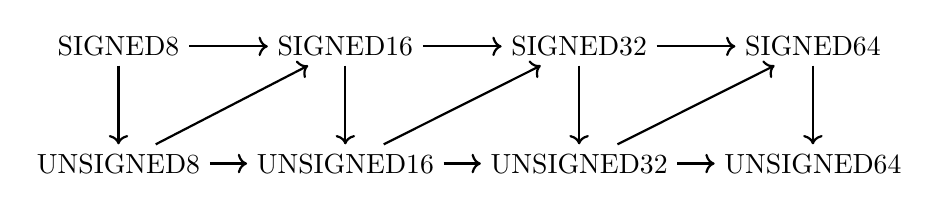
\begin{tikzpicture}
\node (s8) {\SIGNED8};
\node[right = 1cm of s8] (s16)  {\SIGNED16};
\node[right = 1cm of s16] (s32) {\SIGNED32};
\node[right = 1cm of s32] (s64) {\SIGNED64};
\node[below = 1cm of s8] (u8)   {\UNSIGNED8};
\node[below = 1cm of s16] (u16) {\UNSIGNED16};
\node[below = 1cm of s32] (u32) {\UNSIGNED32};
\node[below = 1cm of s64] (u64) {\UNSIGNED64};
\draw[->,thick] (s8) to (s16);
\draw[->,thick] (s16) to (s32);
\draw[->,thick] (s32) to (s64);
\draw[->,thick] (u8) to (u16);
\draw[->,thick] (u16) to (u32);
\draw[->,thick] (u32) to (u64);
\draw[->,thick] (s8) to (u8);
\draw[->,thick] (s16) to (u16);
\draw[->,thick] (s32) to (u32);
\draw[->,thick] (s64) to (u64);
\draw[->,thick] (u8) to (s16);
\draw[->,thick] (u16) to (s32);
\draw[->,thick] (u32) to (s64);
\end{tikzpicture}
\end{center}

\caption{Integer Compatibilities}\label{figure:base types compatibility}
\end{figure}

The range of the larger type includes the ranges of the smaller types.
The smaller type is said to be \emph{compatible} with the larger one in the sense that it can without danger of loss of leading digits be converted.
In assignments and in expansions the conversion of internal representations is automatic.

\emph{Unsigned integers} are compatible with signed or unsigned integer of same or smaller size.
This implies that the assignment from a signed to an unsigned integer of same size is considered ok.
The other direction does not work:

Although the \verb+SIZE+ type is signed and \verb+ADDRESS+ is unsigned,  \verb"SIZE" and \verb"ADDRESS" types are assignment compatible in both directions.

Moreover, integer types are compatible to floating point types, i.e.\ any integer type can be assigned to \FLOAT32 or \FLOAT64\ and \FLOAT32 is compatible to \FLOAT64.

Where there is no implicit compatibility between types, they can be converted with an explicit conversion.
The type name itself can be used for a type conversion.

\begin{annotation}
\subsubsection{Examples}
\begin{lstlisting}[style=example]
VAR
	s8: SIGNED8; s16: SIGNED16; s64: SIGNED64;
	u8: UNSIGNED8; u16: UNSIGNED16; u64: UNSIGNED64;
	adr: ADDRESS; size: SIZE;
BEGIN
	s16 := s8; (* ok *)
	u16 := s8; (* ok *)
	s16 := u8; (* ok *)
	u16 := s16; (* ok *)
	adr := size; (* ok *)
	size := adr; (* ok *)

	s16 := u16; (* error *)
	s16 := SIGNED16(u16); (* ok *)
\end{lstlisting}

\subsubsection{Difference to original Oberon}
The original Oberon fundamental types comprised four integer types \lstinline"SHORTINT", \lstinline"INTEGER", \lstinline"LONGINT" and \lstinline"HUGEINT".

In the early days of Oberon, it was believed by many developers that the type sizes would grow with the hardware.
Effectively, however, the types were fixed to sizes of 8, 16, 32 and 64 bit because a substantial amount of libraries had made assumptions on the implemented type sizes and changing the sizes would have have broken them.

Unfortunately, types that express hardware-dependent properties, such as the address width, were not included, which made it hard to port Oberon to, for example, 64-bit architectures.
Already addresses in the higher 2G of 32-bit systems made problems because they were represented with \lstinline"LONGINT", a signed 32-bit integer type.

We decided to make a radical step and to abandon the old types names completely and to introduce types with type-names that clearly document that they are either bound to a certain bit-width or to features of the hardware.

We introduced unsigned integer types because they can come handy and because they behave different for fundamental operations such as shifts or comparisons.

\paragraph{When to use \SIZE} The type \SIZE\ is the signed analogon of type \ADDRESS.
While type \ADDRESS\ is primarily designed for low-level programming, type \SIZE\ is of high relevance in all kinds of programs.

\SIZE\ must be used when any kind of memory size or interval is (implicitly) addressed.
This implies the use for the lenght of an array, iterating or counting array elements but also iterating or counting elements in other dynamic data structures.

\paragraph{When to use \INTEGER} The type \INTEGER\ represents the word-size of the underlying architecture.
As such, no assumptions on the bit-width of this type should be made.
There are platforms with quite some difference between the address width and the optimal width for integer computation.
For AMD64, for example, the machine word size is defined as 32-bit.

A programmer usually needs to pay attention to some aspects of the internal representation of a type, even if it is only a certain intuition about the types that he or she is using.

A programmer can hope that the word size of a machine matches the typical application domain ("is useful") for generic integers that do not constitute addresses or address differences.
This is the case for "int" in C and it should and probably will be for \INTEGER\ in this dialect of Oberon.

However, we think that the use of \INTEGER\ is quite restricted.
It is certainly useful in education, for rapid prototyping or for any case where the programmer can expect that the result of a computation will be reasonably small for the typical application domain on a given machine.
In all other cases, a programmer needs to use a type with size guarantees (e.g.\ \SIGNED64), the type \SIZE or use a declared type to be flexible.

\paragraph{Use Type Declarations} We generally believe that in the same way as it is good practice to use meaningful variable names, the use of declared types with meaningful type names (such as, "Velocity" or "Amount" or "Bitwidth") provides a good way to document the intended purpose of a type.

\end{annotation}

\subsection{Array Types}
An array is a structure consisting of a number of elements which are all of the same type, called the \emph{element type}.
The number of elements of an array is called its length.
The elements of the array are designated by indices, which are integers between 0 and the length minus 1.

Arrays can be declared in the following form:
\begin{lstlisting}[language = ebnf]
ArrayType = 'ARRAY' [Expression {',' Expression}] 'OF' Type.
\end{lstlisting}

There are two kinds of arrays possible:
\begin{enumerate}
\renewcommand{\labelenumi}{(\alph{enumi})}
\item \emph{Static Arrays} being declared as \ARRAY\ x \OF\ type, where x must be a constant expression,
\item \emph{Open Arrays} being declared as \ARRAY\ \OF\ type.
Open arrays are restricted to pointer base types, element types of open array types, and formal parameter types.
\end{enumerate}
The expression \ARRAY\ x,y \OF\ type is an abbreviatory notation for \ARRAY\ x \OF\ \ARRAY\ y \OF\ type.

Semantic rules:
\begin{itemize}
\item Static arrays of open arrays are not permitted.
\item Arrays of mathematical arrays are not permitted.
\item A length expression \verb~x~ in \ARRAY\ \verb~x~ \OF\ type must be a constant, positive integer or zero
\end{itemize}

\begin{lstlisting}[style=example]
TYPE
	Vector = ARRAY 4 OF REAL;
	Matrix = ARRAY 4,4 OF REAL;
VAR
	buffer: ARRAY 16 OF SIZE;

PROCEDURE Print(CONST x: ARRAY OF CHAR)
\end{lstlisting}

\subsection{Math Arrays}

Special mathematical types have been added to the Oberon language recently.
They can be declared as in
\begin{lstlisting}[style = ebnf]
MathArrayType  = 'ARRAY' '[' MathArraySize {',' MathArraySize} ']' 'OF' Type.
MathArraySize  = Expression | '*' | '?'.
\end{lstlisting}

There are three forms of mathematical arrays possible
\begin{enumerate}
\renewcommand{\labelenumi}{(\alph{enumi})}
\item \emph{Static Mathematical Arrays} being declared as \ARRAY\ $[x]$ \OF\ type, where x must be a constant,
\item \emph{Open Mathematical Arrays} being declared as \ARRAY\ $[*]$ \OF\ type,
\item \emph{Tensors} being declared as \ARRAY\ $[?]$ \OF\ type,
\end{enumerate}
Again, the expression \ARRAY\ \verb~[x,y]~ \OF\ type is an abbreviatory notation for \ARRAY\ \verb~[x]~ \OF\ \ARRAY\ \verb~[y]~ \OF\ type.

Semantic rules:
\begin{itemize}
\item Mathematical arrays of (conventional) arrays are not permitted.
\item Arrays of Tensors and Tensors of Arrays are not permitted.
\item Static Mathematical Arrays of Open Mathematical Arrays or Static Mathematical Arrays of Tensors are not permitted.
\item A length expression \verb~x~ in \ARRAY\ \verb~[x]~ \OF\ type must be a constant, positive integer or zero
\end{itemize}

Math arrays are considered \emph{value types}.
This implies that in an assignment \lstinline"a := b" the data from b are \emph{copied} to a.
If a is an \emph{open} mathematical array, then memory will automatically allocated.
Mathematical arrays can thus also be used to declare open arrays.
An open mathematical array is always initialized with lengths zero.
A tensor is a mathematical array that not only has variable lenghts but even variable dimensions are possible.
It is initialized with dimension 0.
Lengths and dimension of mathematical arrays can be determined with the builtin functions \lstinline"LEN" and \lstinline"DIM".
The length and dimensions of a mathematical array can be set with the \lstinline"NEW" operation.

\begin{annotation}
\subsubsection{Examples}
\begin{lstlisting}[style=example]
VAR
	x: ARRAY [*] OF REAL;
	vec: ARRAY [4] OF REAL;
	matrix: ARRAY [*,*] OF REAL;
	array3: ARRAY [*,3] OF REAL;
	tensor: ARRAY [?] OF FLOAT32;
BEGIN
	NEW(x,5);  (* x has now length 5 *)
	vec := x[0..3]; (* vec now has the content of x *)
	matrix := [x,x]; (* matrix of size 2 x 5 *)
	tensor := FLOAT32(matrix); (* tensor has dimension 2 *)
\end{lstlisting}
\end{annotation}

\subsection{Record Types}

A record type is a structure consisting of a fixed number of elements, called fields, with possibly different types.
The record type declaration specifies the name and type of each field.
The scope of the field identifiers extends from the point of their declaration to the end of the record type, but they are also visible within designators referring to elements of record variables.
If a record type is exported, field identifiers that are to be visible outside the declaring module must be marked.
They are called public fields; unmarked elements are called private fields.

\begin{lstlisting}[style = ebnf]
RecordType = 'RECORD' ['(' QualifiedIdentifier ')']
            [VariableDeclaration {';' VariableDeclaration}]
            {ProcedureDeclaration [';']| OperatorDeclaration [';']}
            'END'.
\end{lstlisting}

\begin{annotation}
\subsubsection{Examples}
\begin{lstlisting}[style=example]
TYPE
    Date = RECORD
        day*, month*, year*: INTEGER
    END

VAR
    x: RECORD
        name, firstname: ARRAY 32 OF CHAR;
        age: INTEGER;
        salary: REAL
    END
\end{lstlisting}
\end{annotation}

Record types are extensible, i.e. a record type can be declared as an extension of another record type.
In the example
\begin{lstlisting}[style=example]
    T0 = RECORD x: INTEGER END
    T1 = RECORD (T0) y: REAL END
\end{lstlisting}
T1 is a (direct) extension of T0 and T0 is the (direct) base type of T1.
An extended type T1 consists of the fields of its base type and of the fields which are declared in T1.
All identifiers declared in the extended record must be different from the identifiers declared in its base type record(s).

Semantic rules
\begin{itemize}
\item The base type \verb~T0~ of a record \verb~T1~ must be a record if the record is defined in the form
    \pc{T1 = RECORD (T0) ... END}.
\item If a type \verb~T1~ is defined as pointer to a record in the form
    \pc{T1 = POINTER TO RECORD (T0) ... END}, then T0 may be a record or a pointer to a record.
\end{itemize}

A record can be marked with the \texttt{FINAL} modifier in which case it cannot be extended:


\begin{annotation}
\subsubsection{Examples}
\begin{lstlisting}[style=example]
TYPE
    Date = RECORD {FINAL}
        day, month, year: INTEGER;
    END
\end{lstlisting}
\end{annotation}

\subsection{Pointer Types}
Formally, pointers can be defined in the form
\begin{lstlisting}[style= ebnf]
PointerType = 'POINTER' [Flags] 'TO' Type.
\end{lstlisting}

Variables of a pointer type \lstinline"P" assume as values pointers to variables of some type \lstinline"T".
T is called the pointer base type of \lstinline"P" and must be a record or array type, unless \lstinline"P" is an unsafe pointer (cf.\ below).
Pointer types inherit the extension relation of their pointer base types: if a type \lstinline"T1" is an extension of \lstinline"T", and \lstinline"P1" is of type \lstinline"POINTER TO T1", then \lstinline"P1" is also an extension of \lstinline"P".


There are thus actually two kinds of (safe) pointers possible in the Active Oberon language:
\begin{enumerate}
\renewcommand{\labelenumi}{(\alph{enumi})}
\item \emph{Pointer to array} being declared as \POINTER\ \TO\ array type
\item \emph{Pointer to record} being declared as \POINTER\ \TO\ record type
\end{enumerate}

If p is a variable of type \lstinline"P = POINTER TO T", a call of the predeclared procedure \lstinline"NEW(p)" allocates a variable of type \lstinline"T" in free storage.
If \lstinline"T" is a record type or an array type with fixed length, the allocation has to be done with \lstinline"NEW(p)";
if \lstinline"T" is an n-dimensional open array type the allocation has to be done with \lstinline"NEW(p, e0, ..., en-1)" where \lstinline"T" is allocated with lengths given by the expressions e0, ..., en-1.
In either case a pointer to the allocated variable is assigned to \lstinline"p". \lstinline"p" is of type \lstinline"P".
The referenced  variable \verb"p^" (pronounced as p-referenced) is of type \lstinline"T".

Any pointer variable may assume the value \NIL, which points to no variable at all.
All pointer variables inherit the extension relation of the basetype \ANY\ and are initialized to NIL.

For systems programming, the Oberon language discussed herein contains unsafe pointers.
An unsafe pointer is assignment compatible to type \ADDRESS\ and pointer arithmetics are allowed.


\begin{annotation}
\subsubsection{Examples}
\begin{lstlisting}[style=example]
CONST
	GPIO = 03F200000H;
VAR
	gpio*: POINTER {UNSAFE} TO RECORD
		GPFSEL: ARRAY 6 OF SET32;
		reserved: ADDRESS;
		GPFSET: ARRAY 2 OF SET32;
		GPFCLR: ARRAY 2 OF SET32;
	END;

BEGIN
	gpio := GPIO;
\end{lstlisting}
\end{annotation}

\subsection{Procedure Types}

Variables of a procedure type T have a procedure (or NIL) as value.
If a procedure \verb"P" is assigned to a variable of type \verb"T", the formal parameter lists of \verb"P" and \verb"T" must match. \verb"P" must not be local to another procedure.
If \verb"P" is a type bound procedure, then \verb"T" must be flagged as delegate.

\begin{lstlisting}[style=ebnf]
ProcedureType = 'PROCEDURE' [Flags] [FormalParameters].
\end{lstlisting}

\begin{annotation}
\subsubsection{Examples}
\begin{lstlisting}[style=example]
TYPE
 Sender* = PROCEDURE {DELEGATE} ( CONST buf: ARRAY OF CHAR; ofs, len: SIZE);
VAR
 Available*: PROCEDURE ( dev: Device ): LONGINT;
\end{lstlisting}
\end{annotation}

\subsection{Object Types}

Objects are basically \emph{pointers to} records that can be equipped with procedures.
Procedures in an object are methods: they reside in the object scope and have access to the object's variables.
An object can be explicitly referred to in its method using the \lstinline"SELF" identifier.

A method prefixed by an ampersand character $\&$ is an \emph{object initializer}.
This method is automatically called when an instance of the object is created and processed before the object becomes publicly available.
An object may have at most one initializer.
If absent, the initializer of the base type is inherited.
Initializers can be called like methods.

Objects can have a body.
This body is executed after the initializer.
A body of an object can be \emph{active}, in which case the body of the object is executed on a separate thread.


\begin{annotation}
\subsubsection{Examples}
\begin{lstlisting}[style=ebnf]
ObjectType = 'OBJECT'
           | 'OBJECT' [Flags] ['(' QualifiedIdentifier ')']
               DeclarationSequence
             [Body]
             'END' [Identifier].
\end{lstlisting}
\end{annotation}

\subsection{Enumeration Types}

An \lstinline"ENUM" type declares a set of scoped constant values called enumerators.
The use of enumeration types provides for type safety by ensuring that invalid values cannot be used for any variable or parameter of an enumeration type involving operations on variables of that type.

The type of an enumerator is the containing enumeration which supports assignment and all ordering relations.
An enumeration can also be extended in which case variables of this type and all of its enumerators become compatible to extending enumerations.
In order to access an enumerator, its name has to be qualified by the name of an enumeration type definition.

Each enumerator has an ordinal value which can be explicitly specified using an arbitrary constant integer expression.
If omitted, the ordinal value of an enumerator corresponds to the value of its immediate predecessor incremented by one.
The implicit ordinal value of the first enumerator is either zero or the biggest ordinal value of all extended enumerations incremented by one.
The actual value of an enumerator or enumeration variable can be obtained by using the \lstinline"ORD" operation which yields the smallest integer type capable of representing all ordinal values of the corresponding enumeration.


Individual identifiers of an ENUM type list can be exported by marking them with \lstinline"*".

\begin{lstlisting}[style=ebnf]
EnumerationType = 'ENUM' ['('QualifiedIdentifier')']
                    IdentifierDefinition ['=' Expression]
                    {',' IdentifierDefinition ['=' Expression]}
                  'END'.
\end{lstlisting}

An \lstinline"ENUM" type may be defined as an extension of an existing ENUM type declaration by including identifier of the base type in the type definition of the extending type.
All enumerated values of the base type become valid values of the new type.
But note that the base type is only downwards compatible with any extended types derived from it, extensions are not upwards compatible with their base type.
This restriction exists because any value of the base type is always a legal value of any extension type derived from it, however not every value of an extension type is also a valid value of the base type.


\begin{annotation}
\subsection{Examples}

Suppose that a variable of enumeration type is exported from a module

\begin{lstlisting}[style=example]
  MODULE Graphics;
  TYPE
    Monochrome* = ENUM
      black*, white* (* ORD(black) has the value 0*)
    END;
  VAR
    pixel* : Monochrome;            (* pixel is exported *)
\end{lstlisting}

After importing the variable it can be used

\begin{lstlisting}[style=example]
  MODULE Application;
  IMPORT Graphics;
  VAR pixel: Graphics.Monochrome;
  BEGIN
    pixel := Monochrome.white; (* qualified *)
\end{lstlisting}

And the enumeration type can be extended, based on the original type

\begin{lstlisting}[style=example]
  TYPE
   Monochrome = Graphics.Monochrome;
   ColourRGB =  ENUM (Monochrome)
   	red, blue, green
   END;
   ColourCYM = ENUM (Monochrome)
   	cyan, yellow, magenta
   END;

  VAR a:Monochrome; b,d: ColourRGB, c: ColourCYM;
    BEGIN
      (* the following are valid, compatible for assignment *)
      a:= ColourRGB.white;
      b:= ColourRGB.blue;
      c:= ColourRGB.yellow;
      b:= a (*valid - value of b is now white *);
      d:= b (*valid - value of d is now blue *);
      (* the following are invalid due to type mismatch *)
      a:= b (*invalid*)
      b:= c (*invalid*)
\end{lstlisting}

\subsubsection{Comparison to original Oberon}
The original Oberon did not feature enumeration types at all and they were added to the language.

Two main objections have previously been levelled against enumeration types:
Potential ambiguity of naming when importing an enumeration type from another module and lack of type extensibility.
To provide a simple solution to the potential ambiguity problem all enumeration identifiers are qualified with the identifier of the type.
The maximum number of identifiers in an enumeration and the value that can be assigned to them is implementation dependent.

In a language without enumeration types, or with “quasi” enumeration types programmers must manually check that values are not out of range, but for large programs this becomes practically impossible, even for small programs it is difficult.
For example the source of the Oberon System is littered with groups of CONST declarations which provide a typeless and error prone substitute for enumeration types.
\end{annotation}

\subsection{Active Cells: Cell Types, Cellnet Types and Port Types}

\begin{lstlisting}[style=ebnf]
CellType = ('CELL' | 'CELLNET') [Flags] [PortList] [';'] {ImportList}
             DeclarationSequence
           [Body] 'END' [Identifier].

PortList = [PortDeclaration {';' PortDeclaration}].

PortDeclaration = Identifier [Flags] {',' Identifier [Flags]}':' PortType.

PortType = 'PORT' ('IN'|'OUT') ['(' Expression ')'].

\end{lstlisting}

\section{Variable Declarations}

Variable declarations introduce variables by defining an identifier and a data type for them.
Variables can be initialized with a value.
If they are not initialized, the initialization with a null value is guaranteed for pointers and otherwise it depends on the implementation of the compiler.

\begin{lstlisting}[style=ebnf]
VariableDeclaration = VariableNameList [':' Type].
VariableNameList = VariableName {"," VariableName}.
VariableName = IdentifierDefinition [Flags]
                [':=' Expression | 'EXTERN' Expression].
Flags = '{' [ Flag {',' Flag} ] '}'.
Flag = Identifier ['(' Expression ')' | '=' Expression].
\end{lstlisting}

Variables can be marked as \lstinline"EXTERN" in which case their identifier is just an alias for a fixed memory location.
This address may be specified by a constant expression or a string literal referring to an entity which is defined elsewhere.
Since extern variables just refer to some other data they cannot be initialized.

The types of the listed variables can be omitted when initializers are present and the type should be inferred from the types.

\subsubsection{Variable initialization}
Variables with an initializer are initialized before they can be used.
Usually, this implies that the initialization is done at the beginning of the respective code section:
\begin{itemize}
\item If a variable is a field in an object, it is initialized after the allocation of the object but before the initializer of the object is called.
\item If a variable is a field in a record, it is initialized when the record is initialized.
\item If a variable is declared in a procedure scope, it is initialized at the beginning of the procedure body.
\item If a variable is declared in a module scope and if the initializer is not a constant expression, it is initialized at the beginning of the module body.
If a variable is declared in a module scope and if the initializer is a constant expression, the variable is initialized in the object file of the module.
This can be important for low-level system module where code (e.g. procedures with flags \lstinline"OPENING") could be executed before the module body.
\end{itemize}

\begin{annotation}
\subsubsection{Examples}
\begin{lstlisting}[style=example]
VAR
	a : REAL;
	b := 10, c : INTEGER;
	c* {UNTRACED} : POINTER TO ARRAY OF CHAR;
	d EXTERN "BaseTypes.Pointer" : ADDRESS;
	e := SomeProc(); (* type inferred *)
\end{lstlisting}



\subsubsection{Difference to original Oberon}
The \lstinline"EXTERN" flag was not present in Original Oberon. Moreover, we have added variable initializers and type inference from the expression type.
\end{annotation}

\section{Procedure Declarations}

A procedure declaration consists of a procedure heading and a procedure body.
The heading specifies the procedure identifier and the formal parameters.
For type-bound procedures it also specifies the receiver parameter.
The body contains declarations and statements.
The procedure identifier is repeated at the end of the procedure declaration.

There are two kinds of procedures: proper procedures and function procedures.
The latter are activated by a function designator as a constituent of an expression and yield a result that is an operand of the expression.
Proper procedures are activated by a procedure call.
A procedure is a function procedure if its formal parameters specify a result type.
The body of a function procedure must contain a return statement which defines its result.

All constants, variables, types, and procedures declared within a procedure body are local to the procedure.
Since procedures may be declared as local objects too, procedure declarations may be nested.
The call of a procedure within its declaration implies recursive activation.

In addition to its formal parameters and locally declared objects, the objects declared in the environment of the procedure are also visible in the procedure (with the exception of those objects that have the same name as an object declared locally).

\begin{lstlisting}[style=ebnf]
ProcedureDeclaration = 'PROCEDURE' ['^'|'&'|'~'|'-'|Flags ['-']]
                       ['(' ParameterDeclaration ')']
                        IdentifierDefinition [FormalParameters]
                        ['EXTERN' Expression ';' | ';'
                        DeclarationSequence  [Body]
                        'END' Identifier].

FormalParameters = '(' [ParameterDeclaration {';' ParameterDeclaration}] ')'
                        [':' [Flags] Type].

ParameterDeclaration = ['VAR'|'CONST'] Identifier [Flags] ['=' Expression]
						{',' Identifier [Flags] ['=' Expression]} ':' Type.

Body = 'BEGIN' [Flags] StatementSequence ['FINALLY' StatementSequence]
						| 'CODE' Code.
\end{lstlisting}

Procedures can be marked as \lstinline"EXTERN" in which case their identifier is just an alias for a fixed memory location.
This address may be specified by a constant expression or a string literal referring to an entity which is defined elsewhere.
Since extern procedures just refer to some other code they do not have a body.


\begin{annotation}
\subsubsection{Examples}
In the following some examples of a procedure declaration are shown.
The last (right most) formal parameters of a procedure can be associated with a default value.
The procdure can then be called with less actual parameters and the remaining formal parameters take on the default values.
If a procedure declaration specifies a receiver parameter (as in the third example below), the procedure is considered to be bound to a type (here: type Student).

\begin{lstlisting}[style=example]
PROCEDURE Send*(CONST data: ARRAY OF CHAR; ofs,len: SIZE;VAR res: INTEGER );
BEGIN (* ... *)
END Send;

PROCEDURE & Init*(scanner: Scanner.Scanner; diagnostics: Diagnostics);
BEGIN (* ... *)
END Init;

PROCEDURE Float*(x: FLOAT64; n := 4, f := 3, d := 0: INTEGER);
BEGIN
	Commands.GetContext().out.FloatFix(x,n,f,d);
END Float;


PROCEDURE (CONST s: Student) GetGrade(Subject: INTEGER): REAL;
BEGIN (* ... *)
END GetGrade;
\end{lstlisting}
\end{annotation}

If a procedure declaration specifies a receiver parameter, the procedure is considered to be bound to a type (see \ref{subsection:Type Bound Procedures}).

\subsection{Formal Parameters}\label{subsection: Formal Parameters}
Formal parameters are identifiers declared in the formal parameter list of a procedure.
They correspond to actual parameters specified in the procedure call.
The correspondence between formal and actual parameters is established when the procedure is called.
There are two kinds of parameters, value and variable parameters, indicated in the formal parameter list by the absence or presence of the keyword VAR.
Value parameters are local variables to which the value of the corresponding actual parameter is assigned as an initial value.
Variable parameters correspond to actual parameters that are variables, and they stand for these variables.
The scope of a formal parameter extends from its declaration to the end of the procedure block in which it is declared.
A function procedure without parameters must have an empty parameter list.
It must be called by a function designator whose actual parameter list is empty too.
The result type of a procedure can be neither a record nor an array.

Let Tf be the type of a formal parameter f and Ta the type of the corresponding actual parameter a.
a needs to be compatible to f in a procedure calls.
Compatibility rules are defined in \ref{subsection: Parameter Compatible}.


\subsection{Type Bound Procedures}\label{subsection:Type Bound Procedures}

Globally declared procedures may be associated with a record type declared in the same module.
The procedures are said to be \emph{bound to} the record type.
The binding is expressed by the type of the receiver in the heading of a procedure declaration.
The receiver may be either a variable or const parameter of record type \lstinline"T" or a value parameter of type \lstinline"POINTER TO T" (where \lstinline"T" is a record type).
The procedure is bound to the type \lstinline"T" and is considered local to it.

If a procedure P is bound to a type $T_0$, it is implicitly also bound to any type $T_1$ which is an extension of $T_0$.
However, a procedure $P'$ (with the same name as $P$) may be explicitly bound to $T_1$ in which case it \emph{overrides} the binding of $P$. $P'$ is considered a redefinition of $P$ for $T_1$.
The signature of $P$ and $P'$ must match (see \ref{subsection: Matching Signature}).
If $P$ and $T_1$ are exported  $P'$ must be exported too.

If $v$ is a designator and $P$ is a type-bound procedure, then \lstinline"v.P" denotes that procedure $P$ which is bound to the \emph{dynamic type} of $v$.
Note, that this may be a different procedure than the one bound to the static type of $v$. $v$ is passed to $P$'s receiver according to the parameter passing rules specified in Section \ref{subsection: Formal Parameters}.


If $r$ is a receiver parameter declared with type $T$, \lstinline"r.P^" denotes the (redefined) procedure $P$ bound to the \emph{base type} of $T$.
The signature of both declarations must match (\ref{subsection: Matching Signature}).

\begin{annotation}
\subsubsection{Examples}
\begin{lstlisting}[style=example]
PROCEDURE (t: Tree) Insert (node: Tree);
  VAR p, father: Tree;
BEGIN p := t;
  REPEAT father := p;
    IF node.key = p.key THEN RETURN END;
    IF node.key < p.key THEN
      p := p.left
    ELSE
      p := p.right
    END
  UNTIL p = NIL;
  IF node.key < father.key THEN
    father.left := node
  ELSE
    father.right := node
  END;
  node.left := NIL; node.right := NIL
END Insert;

PROCEDURE (t: CenterTree) Insert (node: Tree);  (*redefinition*)
BEGIN
  WriteInt(node(CenterTree).width);
  t.Insert^ (node)  (* calls the Insert procedure bound to Tree *)
END Insert;

PROCEDURE (t: TreeNodePointer) Copy (): TreeNodePointer;  (
VAR c: TreeNodePointer;
BEGIN
	NEW(c); (* ... *)
	RETURN c;
END Copy;

PROCEDURE (t: CenterTreeNodePointer) Copy (): TreeNodePointer;  (
VAR c: CenterTreeNodePointer;
BEGIN
	NEW(c); (* ... *)
	RETURN c;
END Copy;

\end{lstlisting}

\begin{remark} Note that the type of a receiver parameter can decide about the dynamic nature of the object that can receive a procedure call.
It the receiver type is a pointer type, then the procedure can only be called on an object on the heap.
If the receiver is a record type, then the procedure can be called on both, heap and stack, and it is not possible that the heap pointer escapes from the type.

Constness of records: Naturally, if a variable of record type is const, only receivers with a const parameter can receive a call.
This ensures that the const property of a record can not be undermined by a call to a type bound procedure.
\end{remark}

\end{annotation}

\begin{annotation}
\subsection{Oberon-2}

The explicit receiver for type bound procedures allows to distiguish between procedures that modify the respective object and those that let it unchanged. In C++ this is solved by adding a \lstinline"const" modifier at member functions:
\begin{lstlisting}[style=example,language=C]
class Counter {
private:
  unsigned int value = 0;
public:
  void increment (unsigned by){
    value += by;
  }
  unsigned current() const {
    return value;
  }
}
\end{lstlisting}

With type bound procedures, the same kind of semantics can be very naturally designated with the \lstinline"var" / \lstinline"const" modifiers of the receiver parameter:
\begin{lstlisting}[style=example]
TYPE Counter* = RECORD value: UNSIGNED64 END;

PROCEDURE (VAR c: Counter) Increment (by: UNSIGNED64);
BEGIN
	INC(c.value, by);
END Increment;

PROCEDURE (CONST c: Counter) Current (): UNSIGNED64;
BEGIN
	RETURN c.value;
END Increment;

\end{lstlisting}

Moreover, the nomenclature very naturally describes what happens during a call to the methods, namely that the receiver object is passed as implicit parameter to the procedure.
\begin{lstlisting}[style=example]
VAR c: Counter;
c.Increment(10); // c is passed as variable parameter
...
ASSERT(c.Current()>=10); // c is passed as const parameter
\end{lstlisting}

Classes in C++ are generally value types and they can be allocated on heap (with \lstinline"new") or stack (implicitly).
Pointer to structs / classes can point into heap or stack.
Pointers are not protected in this sense.

In Oberon, (safe) pointers are, by definition, limited to the heap.
It is impossible to create a pointer to a stack object.
This implies a limitation: record types cannot be transformed to a pointer
In order to allow to create complex data structures of objects that are implemented using an object-oriented approach, in Active Oberon the concept of an \lstinline"OBJECT" has been introduced. Objects invariantly live on the heap.
Syntactically, methods on objects were defined in the object's scope. Very much like it is done in Java.
We identified a strong drawback of this approach: every object needs to be allocated on the heap, even if its lifetime is very much limited.
This, in turn, creates a high pressure on the garbage collector and makes it harder to come up with a system without garbage collection at all.
One idea (merely on the syntactical level) was to replace \lstinline"OBJECT" by \lstinline"RECORD" and to allow to write the type bound procedures within the record.
Such methods would, by default, be allowed to change the object content, i.e.\ be implemented with an implicit \lstinline"VAR" receiver:

The code
\begin{lstlisting}[style=example]
TYPE
Counter* = RECORD
  value: UNSIGNED64

  PROCEDURE Increment (by: UNSIGNED64);
  BEGIN
    INC(value, by);
  END Increment;

  PROCEDURE Current (): UNSIGNED64;
  BEGIN
    RETURN value;
  END Increment;
END;
\end{lstlisting}
would be implemented, implicitly, as
\begin{lstlisting}[style=example]
TYPE Counter* = RECORD value: UNSIGNED64 END;

PROCEDURE (VAR SELF: Counter) Increment (by: UNSIGNED64);
BEGIN
	INC(value, by);
END Increment;

PROCEDURE (VAR SELF: Counter) Current (): UNSIGNED64;
BEGIN
	RETURN value;
END Increment;
\end{lstlisting}
Of course, it would be possible to add the \lstinline"CONST" keyword somewhere in the definition of the record just as it is done in C++ in order to make a distinction between modifying and non-modifying code.
However, there is another very important reason to stay with the elegant and natural type-bound procedures declaration of Oberon-2:
It is possible to write type bound procedures that can act on a variable of record type (being located on heap or on stack) and to write type bound procedures that can act on a variable of pointer type (being solely located on the heap).
The latter allows to explicitly distinguih between code that can be called on a pointer (and might return the pointer) from code that can only be called on a record.

\begin{lstlisting}[style=example]
TYPE Expression = RECORD END;
TYPE PExpression = POINTER TO Expression;

(* every expression can be evaluated *)
PROCEDURE (e: Expression) Evaluate(): Value; (* ... *)
(* only pointer expressions can be registered *)
PROCEDURE (e: PExpression) Register (); (*...*)
\end{lstlisting}


\end{annotation}
\subsection{Operator Declaration}\label{subsection: Operator Declaration}

Oberon, in the version presented here, supports operator overloading. Operators can be declared in the following way.

\begin{lstlisting}[style=ebnf]
OperatorDeclaration  = 'OPERATOR' [Flags] ['-'] String ['*'|'-'] FormalParameters ';'
                         DeclarationSequence
                         [Body]
                       'END' String.
\end{lstlisting}

At least one of the involved parameters must be defined in the operator defining module.
Overloaded operators are searched in all directly or indirectly loaded modules.
In order to find the operator overloaded for an expression, for each operator a distance is computed.
The first operator found with minimal distance is determined.
If there are operators with the same minimal distance for an expression, the outcome is not uniquely defined.

\section{Expressions}

\subsection{Expression}

Expressions are of the following form:
\begin{lstlisting}[style=ebnf]
Expression = RangeExpression [RelationOp RangeExpression].
RelationOp = '=' | '#' | '<' | '<=' | '>' | '>=' | 'IN' | 'IS'
             | '.=' | '.#' | '.<' | '.<=' | '.>'  '.>='
             | '??' | '!!' | '<<?' | '>>?'.
\end{lstlisting}
The operators in the second and third line of RelationOp are defined specifically for the Math Arrays and Active Cells subset of the language, respectively.

\subsection{Range Expressions}
Range Expressions are defined as follows
\begin{lstlisting}[style=ebnf]
RangeExpression = SimpleExpression
          | [SimpleExpression] '..' [SimpleExpression]['by' SimpleExpression]
          | '*' .
\end{lstlisting}

\subsubsection{Difference to original Oberon}
The notion of Range Expressions has been introduced and thus the ranges used in the Set types has been elevanted to Expressions in order to be able to represent slices in Math Oberon.

\subsection{Simple Expressions}

\begin{lstlisting}[style=ebnf]
SimpleExpression = Term {AddOp Term}.
AddOp            = '+' | '-' | 'or'.
\end{lstlisting}

\begin{annotation}
\subsubsection{Difference to original Oberon}
The unary operator "-" and "+" were originally contained here in the simple expression.
We have moved them to the Factor as we believe it should have higher precedence, similar to the logical not operator.

We found an example of an assertion (in code that was productive): the assertion
\begin{lstlisting}[style=example]
	assert(-1 MOD 3 = -1); (* did not fail, but fails now *)
\end{lstlisting}
was used in order to determine that \lstinline"a MOD 3" would be negative for $a<0$, something that is indeed untrue for Oberon.
In fact, \lstinline"(-1) MOD 3 = 2"!
The assertion held true because \lstinline"-1 MOD 3" used to be \lstinline"-(1 MOD 3)".
\end{annotation}

\subsection{Terms}
\begin{lstlisting}[style=ebnf]
Term  = Factor {MulOp Factor}.
MulOp = '*' | '/' | 'DIV' | 'MOD' | '&'
        | '.*' | './' | '\' | '**' | '+*' .
\end{lstlisting}
The operators defined in the second line of MulOp are defined specifically for Math Arrays.


\subsection{Factors}

Factors are defined as
\begin{lstlisting}[style=ebnf]
Factor = UnaryExpression | UnaryOperation Factor.
UnaryOperation = '~' | '+' | '-'.
\end{lstlisting}


\begin{annotation}
\subsubsection{Difference to original Oberon}
The original Oberon specification contained keywords, literals and designators as parts of the Factor.
We moved this to a separate productions: unary and primary expressions, to avoid ambiguities in the syntax.
\end{annotation}

\subsection{Unary and Primary Expressions}

Primary Expressions constitute expressions that are not combined via free standing binary or prefix-operators but rather formed by a designator, literal, keyword or special structural expression that may be suffixed by further operations such as a procedure call, an index operator, an up-call or dereference operator or selector.

Primary expressions can provide an expression with address (that can stand of the left hand side of an assignment, for instance) or an expression that only has a value.

\begin{lstlisting}[style=ebnf]
UnaryExpression = PrimaryExpression [DesignatorOperations] [Flags].

PrimaryExpression = Number | Character | String | Set | Array
        | 'NIL' | 'IMAG' | 'TRUE' | 'FALSE' |
        | 'SELF' | 'RESULT' | 'ADDRESS' | 'SIZE'
        | 'SIZE' 'OF' Factor | 'ADDRESS' 'OF' Factor
        | 'ALIAS' OF Factor
        | 'NEW' UnaryExpression
        | '(' Expression ')'
        | Identifier.

DesignatorOperations = { "(" [ExpressionList] ")"
                       | "." Identifier
                       | '[' IndexList ']'
                       | '^'
                       | '`'
                    } .

ExpressionList = Expression { ',' Expression }.

IndexList = '?' [',' ExpressionList]
             |  ExpressionList [',' '?' [',' ExpressionList] ]
\end{lstlisting}
The suffix operator "\verb~`~" is defined specifically for Math Arrays.


\begin{annotation}
\subsubsection{Examples}
\begin{lstlisting}[style=example,caption=Example of Designators]
	a[10]
	P(3,5).GetArray[5].CallMe()
	myVariable(Type)
\end{lstlisting}

The \lstinline"RESULT" designator can be used to access the (implicit) return parameter of a procedure return parameter.
This feature was implemented in order to reduce memory pressure in avoiding reallocations of already allocated return parameters.
The statement \lstinline"RETURN RESULT;" only returns from a procedure without writing the result.
The latter can also be used when the return value of a procedure has already been written in inline assembly code.
\begin{lstlisting}[style=example]
PROCEDURE ReturnLargeArray(): ARRAY[*] OF REAL;
BEGIN
	IF LEN(RESULT) < LargeSize THEN
		NEW(RESULT, LargeSize)
	END;
	...
	RETURN RESULT;
END ReturnLargeArray;
\end{lstlisting}

\subsubsection{Difference to original Oberon}
The notion of a Designator, as it was present in previous descriptions of the language, has been replaced by a primary expression.
Due to the more liberal handling of chained expressions like the example shown below, the distinction between expressions that can be used on the left hand side of an assignment operator and expressions that constitute only a value, cannot be made so clear any more.
\begin{lstlisting}[style=example]
expression(BinaryExpression).left.CompatibleTo(x)
\end{lstlisting}

Also, in order to avoid ambiguities in the EBNF, and to allow other features such as type guards on value types (such as literal numbers), we chose to unify such expressions and call them primary expressions.

A type guard on numbers has been introduced.
A guarded number is converted to the given type if and only if its value is not changed.
When it fails (i.e. when the actual value of a number is not compatible to / cannot be represented by the type), a trap is raised.

Complex numbers have beend added to the language.
Therefore the literal 'IMAG' has been introduced.

Because \SIZE\ and \ADDRESS\ are types, the meaning of \lstinline"SIZE(x)" and \lstinline"ADDRESS(y)" (formally \lstinline"SYSTEM.SIZE(x)" and \lstinline"SYSTEM.ADDRESS(x)" has changed.
Therefore, the forms \lstinline"ADDRESS OF" and \lstinline"SIZE OF" have been introduced.

Similarly \lstinline"ALIAS OF" has been introduced for Math Arrays.

Various operators, including the suffix transpose operator "\lstinline~`~" have been introduced for Math Arrays.


In contrast to the original \lstinline"NEW" statement, the designator form \lstinline"NEW Type(parameters)" has been introduced in order to be able to allocate a type and assign it to a base type at the same type.
\begin{lstlisting}[style=example]
VAR
	x: Expression;
BEGIN
	x := NEW BinaryExpression(left, right);
\end{lstlisting}

Moreover, it is now possible to initialize a pointer to record with a call to a procedure returning a record in the form \lstinline"NEW Procedure(parameters)". Also Pointers from record types can be allocated in the form \lstinline"NEW RecordType";

\begin{lstlisting}[style=example]
TYPE
  Student = RECORD
    name: ARRAY 32 OF CHAR;
    age: INTEGER
  END;

  PROCEDURE StudentInstance(CONST name: ARRAY OF CHAR;
                                          age: INTEGER): Student;
  BEGIN
    COPY(name, RESULT.name);
    RESULT.age := age;
    RETURN RESULT;
  END StudentInstance;

(* POINTER TO Student *)
VAR student1 := NEW Student;
VAR student2 := NEW StudentInstance("Niklas",6);
(* Student *)
VAR student3 := StudentInstance("Hannes",9);
\end{lstlisting}

Most of the restrictions to designators were removed.
For example, designators can be arbitrarily chained and references returned from procedure calls can be passed to const parameters.

\begin{lstlisting}[style=example, caption=Example of a syntactially valid designator]
	P(3)[10].p(Q());
\end{lstlisting}

\end{annotation}


\subsection{Operator Table}\label{section:OperatoTable}
For a given operator, the types of its operands are expression compatible if they conform to the following table (which shows also the result type of the expression).
In the following, we assume that T1 is an extension of T0.

\begin{longtable}{p{0.15\linewidth}p{0.2\linewidth}p{0.2\linewidth}p{0.25\linewidth}}
operator & first operand & second operand & result type \\ \hline
\lstinline$+$, \lstinline$-$, \lstinline$*$ &  numeric & numeric & smallest numeric type including both operands\\
\lstinline$/$ & numeric & numeric & smallest \FLOAT-type including both operands\\
\lstinline$+$, \lstinline$-$, \lstinline"*", \lstinline"/" & \SET{n} & \SET{m} & Smallest \SET-type including both operands\\
\DIV, \MOD & integer & integer & smallest integer type including both operands\\
\lstinline"OR",\lstinline"&", \&, $\sim$ & \BOOLEAN & \BOOLEAN & \BOOLEAN\\
\lstinline"=", \lstinline"#", \lstinline"<", \lstinline"<=", \lstinline">", \lstinline">=" & numeric & numeric & \BOOLEAN\\
& \CHAR & \CHAR & \BOOLEAN\\
& character array, string & character array, string& \BOOLEAN\\
\lstinline$=$, \lstinline$#$ & \BOOLEAN & \BOOLEAN & \BOOLEAN\\
& \SET & \SET & \BOOLEAN\\
& \NIL, pointer type T0 or T1 & \NIL, pointer type T0 or T1 & \BOOLEAN \\
& procedure type T, NIL & procedure type T, NIL &  \BOOLEAN\\
\IN & integer & set & \BOOLEAN \\
\IS & T0 & type T1 & \BOOLEAN
\end{longtable}

\section{Statements}

\begin{lstlisting}[style=ebnf]
Statement = [
  UnaryExpression
    [':=' Expression
    | '!' Expression | '?' Expression | '<<' Expresssion | '>>' Expression
    ]
  | 'VAR' Identifier [':=' Expression]
          {',' Identifier [':=' Expression]} [':' Type]
  | 'IF' Expression 'THEN' StatementSequence
    {'ELSIF' Expression 'THEN' StatementSequence}
    ['ELSE' StatementSequence]
    'END'
  | 'WITH' Identifier ':' QualifiedIdentifier 'DO' StatementSequence
    {'|' QualifiedIdentifier 'DO' StatementSequence}
    [ELSE StatementSequence]
    'END'
  | 'CASE' Expression 'OF' ['|'] Case
    {'|' Case}
    ['ELSE' StatementSequence]
    'END'
  | 'WHILE' Expression 'DO'
      StatementSequence
    'END'
  | 'REPEAT'
      StatementSequence
    'UNTIL' Expression
  | 'FOR' Identifier ':=' Expression 'TO' Expression ['BY' Expression] 'DO'
      StatementSequence
    'END'
  | 'LOOP' StatementSequence 'END'
  | 'EXIT'
  | 'RETURN' [Expression]
  | 'AWAIT' Expression
  | StatementBlock
  | 'CODE' {any} 'END'
  | 'IGNORE' Expression
].

Case = RangeExpression {',' RangeExpression} ':' StatementSequence.

StatementBlock = 'BEGIN' [Flags] StatementSequence 'END'.

StatementSequence = Statement {';' Statement}.
\end{lstlisting}

\subsection{Statement Block and Statement Sequences}
Statements may be grouped into a block delimited by BEGIN and END.
The block may include modifiers in braces \lstinline"{}"  which modify the properties of actions within the block.
See individual statement types for details of their modifiers.
A sequence of  more than one statement denotes the sequence of actions specified by the component statements, they are delimited by semicolons.

\begin{lstlisting}[style=ebnf]
StatementBlock = 'BEGIN' [Flags] StatementSequence 'END'.
StatementSequence = Statement {';' Statement}.
\end{lstlisting}

\begin{annotation}
\subsubsection{Examples}
\begin{lstlisting}[style=example]
BEGIN{EXCLUSIVE} (* an exclusive statement block *)
  state := States.normal;
  AWAIT(state = States.alert)
END;
\end{lstlisting}
\end{annotation}


\subsection{Assignment Statement}
The assignment serves to replace the current value of a variable by a new value specified by an expression.
The assignment operator is written as \lstinline":="  and pronounced as \emph{becomes}.

\begin{lstlisting}[style=ebnf]
	UnaryExpression ':=' Expression
\end{lstlisting}

The type of the designator must be assignment compatible with the type of the expression.

\begin{annotation}
\subsubsection{Examples}
\begin{lstlisting}[style=example,caption=Examples of Assignments]
  i := 0;
  x := 3.4;
  y := i*i;
\end{lstlisting}
\end{annotation}

\subsection{Declaration Statement}
\begin{lstlisting}[style=ebnf]
'VAR' Identifier [':=' Expression]
      {',' Identifier [':=' Expression]} [':' Type];
\end{lstlisting}

Variables can be declared within a statement sequence. A declaration statement is indicated by the \lstinline"VAR" keyword. Similar to variable declaration, the type of the variable can be omitted when an initializer is present and when the type of the initializer shall be taken for the variable type. The variable is visible within the statement sequence from the point of declaration to the end of the procedure scope. A variable can only be declared once in a procedure scope.

\begin{annotation}
\subsubsection{Examples}
\begin{lstlisting}[style=example]
BEGIN
	VAR a := 20, b: SIZE; (* both, a and b are of type SIZE *)
	VAR c := a, d := 30; (* c is of type of a and d is SIGNED8 *)
	...
END
\end{lstlisting}

\subsubsection{Difference to original Oberon}
We have introdcued the declaration statement motivated by the need to support a better way of initialization for value (record) types.
\end{annotation}

\subsection{Procedure Call Statement}
A procedure call serves to activate a procedure.
The procedure call may contain a list of actual parameters which are substituted in place of their corresponding formal parameters defined in the procedure declaration.
The correspondence is established by the relative positions of the parameters in the lists of actual and formal parameters respectively.

\begin{lstlisting}[style=ebnf]
	UnaryExpression ["(" ExpressionList ")"];
\end{lstlisting}

There are three kinds of parameters: value, constant and variable parameters.
In the case of variable parameters, the actual parameter must be a designator representing an address.
If it designates an element of a structured variable, the selector is evaluated when the formal/actual parameter substitution takes place, i.e.\ before the execution of the procedure.

If the parameter is a value parameter, the corresponding actual parameter must be an expression.
This expression is evaluated prior to the procedure activation, and the resulting value is assigned to the formal parameter which now constitutes a local variable on the callee side.

If the parameter is a constant parameter, the corresponding actual parameter can be copied but it does not have to.
The compiler can optimize.
This is particularly handy for strings and large records.

\begin{annotation}
\subsubsection{Examples}
\begin{lstlisting}[style=example]
PROCEDURE Test(a: SIGNED32; VAR r: REAL;
                 CONST c: Student; CONST s: ARRAY OF CHAR);
BEGIN
  IF c.semester = 2 THEN (* c might be passed by reference here *)
    a := a * 2; (* no effect to caller *)
    r := 20; (* effect to caller *)
    TRACE(s);
  END;
END Test;

VAR r: REAL;
Test(22, r, student, "Rabbit");
\end{lstlisting}

\subsubsection{Difference to original Oberon}
We have introduced \CONST\ parameters in order to support the read-only access to large arrays in the MathArray framework.
It turned out to be very useful for records and strings also.
\end{annotation}



\subsection{Communication Statement}
The various communication statements are used in the Active Cells subset of the language.
They are used to send and receive data via a port in a blocking or non-blocking way.

\subsection{If-Elsif-Else-End Statement}
An \lstinline"IF" statement specifies the conditional execution of statements depending on the evaluation of a a Boolean expression called its guard.
The guards are evaluated in sequence of occurrence, until one evaluates to \lstinline"TRUE", thereafter its associated statement sequence is executed.
If no guard is satisfied, the statement sequence following the symbol \lstinline"ELSE" is executed, if there is one.

\begin{lstlisting}[style=ebnf]
'IF' Expression 'THEN' StatementSequence
    {'ELSIF' Expression 'THEN' StatementSequence}
    ['ELSE' StatementSequence]
    'END'
\end{lstlisting}

\begin{annotation}
\subsubsection{Examples}
\begin{lstlisting}[style=example]
IF ch <= "9" THEN RETURN ORD( ch ) - ORD( "0" )
ELSIF ch <= "F" THEN RETURN ORD( ch ) - ORD( "A" ) + 10
ELSIF ch <= "f" THEN RETURN ORD( ch ) - ORD( "a" ) + 10
ELSE Error( Basic.NumberIllegalCharacter );  RETURN 0
END
\end{lstlisting}
\end{annotation}



\subsection{Case Statement}
A \lstinline"CASE" statement specifies the selection and execution of a statement sequence according to the value of an expression.
First the case expression is evaluated, then the statement sequence is executed whose case label list contains the obtained value.
The case expression and all labels must be of the same type, which must be an enumeration type, integer type, any \lstinline"SET" type or \lstinline"CHAR".
Case labels are constants, and no value must occur more than once in a single \lstinline"CASE" statement.
If the value of the expression does not occur as a label of any case, the statement sequence following the symbol \lstinline"ELSE" is selected, if there is one.
If, in this situation, there is no \lstinline"ELSE" part, a trap is raised.

\begin{lstlisting}[style=ebnf]
'CASE' Expression 'OF' ['|'] Case
    {'|' Case}
    ['ELSE' StatementSequence]
    'END'
\end{lstlisting}

\begin{annotation}
\subsubsection{Examples}
\begin{lstlisting}[style=example]
CASE ch OF
  EOT: s := EndOfText
  | '#': s := Unequal;  GetNextCharacter
  | '&': s := And;  GetNextCharacter
  | '[': s := LeftBracket;  GetNextCharacter
  | ']': s := RightBracket;  GetNextCharacter
  (* ... *)
ELSE
  s := Identifier;  GetIdentifier( token );
END;
\end{lstlisting}
\end{annotation}

\subsection{With Statement}
When working with a variables $p$ of dynamic type (e.g.\ pointers to records or reference parameters of record type), often it is required to guard $p$ to a type that extends the static type of $p$.
The \lstinline"WITH" statement assumes a role similar to the type guard, extending the guard over an entire statement sequence.
It may be regarded as a regional type guard.

Moreover, the \lstinline"WITH" statement allows to check for a type and conditionally execute a statement sequence depending of the dynamic type.
A \lstinline"WITH" statement can, in this sense, be regarded like a \lstinline"CASE" statement for types.

If the dynamic type of the guarded variable is not of dynamic type of any of the alternatives given, the \lstinline"ELSE" branch is taken.
If no \lstinline"ELSE" branch is present in such cases, a trap will be raised.

\begin{lstlisting}[style=ebnf]
'WITH' Identifier ':' QualifiedIdentifier 'DO' StatementSequence
    {'|' QualifiedIdentifier 'DO' StatementSequence}
    [ELSE StatementSequence]
    'END'
\end{lstlisting}

If a type $T_1$ is referred to by a qualified identifier in the \WITH\ statement and a type $T_2$ is referred to by a later qualified identifier later in the same \WITH, $T_2$ may not extend $T_1$ (otherwise the branch with $T_2$ would never be reachable).

\begin{annotation}
\subsubsection{Examples}
\begin{lstlisting}[style=example, caption=Example of a WITH statement]
WITH x:
| SyntaxTree.ResultDesignator DO result := ResolveResultDesignator(x)
| SyntaxTree.SelfDesignator DO result := ResolveSelfDesignator(x)
| SyntaxTree.BinaryExpression DO result := ResolveBinaryExpression(x)
| SyntaxTree.UnaryExpression DO result := ResolveUnaryExpression(x)
END;
\end{lstlisting}

\begin{lstlisting}[style=example, caption= Example of a rejected WITH statement when UnaryExpression inherits from Expression]
WITH x:
| SyntaxTree.Expression DO (* general case *)
| SyntaxTree.UnaryExpression DO (* forbidden ! *)
END;
\end{lstlisting}

\subsubsection{Difference to original Oberon}
In Oberon-2 the \WITH\ statement with alterantives was present buth then it was removed again.
We reintroduced it in a slighty modified form.
We removed the necessity to repeat the variable name for each case occuring.

It should be noted that, technically, \WITH\ is different from \CASE\ in the following sense.
While for \CASE\ it is relatively straighforward to implement an optimized version with a branch table, this is not the case for \WITH, particularly not with dynamic module loading.
However, at least the indirect loading of the type tags as it would occur in a multi-case \IF\ statement can be avoided here by keeping the type tag address in a register.
This is a simple optimisation that can be implemented with little costs in a compiler.
\end{annotation}

\subsection{While Statement}

A \WHILE\ statement specifies repetition zero or more times of some statements.
If the Boolean expression (guard) yields \TRUE, then the statement sequence is executed.
The expression evaluation and the statement execution are repeated as long as the Boolean expression yields \TRUE.

\begin{lstlisting}[style=ebnf]
'WHILE' Expression 'DO'
    StatementSequence
'END'
\end{lstlisting}

\begin{annotation}
\subsubsection{Examples}
\begin{lstlisting}[style=example]
WHILE len > 0 DO
  data[length] := buf[ofs];
  INC(ofs); INC(length); DEC(len)
END;
\end{lstlisting}
\end{annotation}

\subsection{Repeat-Until Statement}
A \REPEAT\ statement specifies the repeated execution of a statement sequence until the Boolean expression (guard) yields TRUE.
The statement sequence is thus executed one or more times.

\begin{lstlisting}[style=ebnf]
'REPEAT'
    StatementSequence
'UNTIL' Expression
\end{lstlisting}

\begin{annotation}
\subsubsection{Examples}
\begin{lstlisting}[style=example]
REPEAT
  expression := Expression();
  expressionList.AddExpression( expression )
UNTIL ~Optional( Scanner.Comma );
\end{lstlisting}
\end{annotation}
\subsection{For Statement}
The \FOR\ statement provides a means of repeating a sequence of statements for a number of times whilst automatically incrementing or decrementing a variable by a fixed constant value.
The loop continues whilst the value of the \FOR\ variable (counter) is within the range specified by the two expressions.

It is mainly used in arithmetic algorithms where the counter may typically be used as an array index.

\begin{lstlisting}[style=ebnf]
'FOR' Identifier ':=' Expression 'TO' Expression ['BY' Expression] 'DO'
    StatementSequence
'END'
\end{lstlisting}

The for statement is equivalent to a while statement with a additional temporary variable for the end value.
The start and end value of the for-loop are only evaluated once.
The increment of a for-loop must be constant expression.

\begin{lstlisting}[style=example]
FOR i := start TO end BY increment DO
	Statements
END;
\end{lstlisting}
is equivalent to
\begin{lstlisting}[style=example]
i := start;
temp := end;
IF increment > 0 THEN
  WHILE i <= temp DO
    Statements;
    i := i + increment;
  END;
ELSE
  WHILE i >= temp DO
    Statements;
    i := i + increment;
  END;
END;
\end{lstlisting}

\begin{annotation}
\subsubsection{Examples}
\begin{lstlisting}[style=example]
FOR i := 0 TO EndOfText DO ASSERT(symbols[i] # "") END;
\end{lstlisting}
\end{annotation}

\subsection{Loop and Exit Statement}
A \LOOP\ statement specifies the repeated execution of a statement sequence, the loop is terminated by the execution of any \EXIT\ statement within that sequence.



An EXIT statement consists of the symbol EXIT.
It specifies termination of the enclosing loop statement and continuation with the statement following the END of that loop statement.
Each Exit statement is contextually, although not syntactically bound to the loop statement which contains it.

\begin{lstlisting}[style=ebnf]
'LOOP' StatementSequence 'END'
\end{lstlisting}

\begin{annotation}
\subsubsection{Examples}
The use of \WHILE\ and \REPEAT\ statements is recommended for the most cases.
A loop statement can be useful to express repetition where there are several termination conditions at different points in the code.

\begin{lstlisting}[style=example]
LOOP
  IF ("0" <= ch) & (ch <= "9") OR (d = 0) & ("A" <= ch) & (ch <= "F") THEN
    dig[n] := ch;  INC( n ) END;
  ELSIF ch = "." THEN
  	m := n;
  ELSE EXIT
  END
END;
\end{lstlisting}
\end{annotation}

\subsection{Return Statement}
A \RETURN\ statement is used to return from a procedure.
If the procedure is declared to return a value of type $T$, the return statement must return an expression of assignment compatible type.

\begin{annotation}
\subsubsection{Examples}
\begin{lstlisting}[style=example]
PROCEDURE Ten( e: SIGNED32 ): FLOAT64;
VAR x, p: FLOAT64;
BEGIN
  x := 1;  p := 10;
  WHILE e > 0 DO
    IF ODD( e ) THEN x := x * p END;
    e := e DIV 2;
    IF e > 0 THEN p := p * p END  (* prevent overflow *)
  END;
  RETURN x
END Ten;
\end{lstlisting}
\end{annotation}


\subsection{Await Statement}
The \AWAIT\ statement is a statement to synchronize runnning processes (threads).

\begin{lstlisting}[style=ebnf]
'AWAIT' Expression
\end{lstlisting}


\subsection{Code Block}
Code Blocks can be used in order to write inline assembly code in Oberon.
\begin{lstlisting}[style=ebnf]
'CODE' {any} 'END'
\end{lstlisting}

\begin{annotation}
\subsubsection{Examples}
\begin{lstlisting}[style=example]
OPERATOR -"-"*(x {REGISTER}: Vector): Vector;
VAR res{REGISTER}: Vector;
BEGIN
  CODE
    XORPS res, res
    SUBPS res, x
  END;
  RETURN res;
END "-";
\end{lstlisting}
\end{annotation}

\subsection{Ignore Statement}
The \IGNORE\ statement can be used in order to ignore the result of a procedure call.

\begin{lstlisting}[style=ebnf]
'IGNORE' Expression
\end{lstlisting}

\begin{annotation}
The \IGNORE\ statement was introduced for interfacing with C libraries, where often the result of a library call is ignored.
It was not present in the original Oberon.

\subsubsection{Examples}
\begin{lstlisting}[style=example]
IGNORE User32.SetWindowText(root.hWnd, windowTitle);
IGNORE User32.BringWindowToTop( root.hWnd );
IGNORE User32.SetForegroundWindow( root.hWnd );
\end{lstlisting}

It turned out to be also convenient for supporting passing on results in chained stream-expressions, as they are, for example, available in C++.
\begin{lstlisting}[style=example]
IGNORE Out.GetWriter() << "This is text " << "that is concatenated";
\end{lstlisting}

\end{annotation}

\section{Built-in Functions and Symbols}
There are some built-in procedures and functions in Active Oberon.
We give a short overview in the following table.
Note that Integer stands for \SIGNED{x} or \UNSIGNED{x}, \SIZE\ or \INTEGER\.
Float stands for any of \FLOAT{x} or \REAL.
Number stands for Integers or Float.
Set stands for any of \SET{x} or \SET.
Complex stands for any of \COMPLEX{x} or \COMPLEX.
\subsection{Global}
\subsubsection{Conversions}
\begin{longtable}{|p{0.25\linewidth}|p{0.2\linewidth}|p{0.15\linewidth}|p{0.25\linewidth}|}
\hline
Function & Argument Types & Result Type & Description \\
\hline\hline
\endhead
ABS(x) & x: Number & Number & return absolute value of x\\
CAP(x) & x: CHAR & CHAR & return capital letter of x\\
CHR(x) & x: Integer & CHAR & return character with ascii-number x\\
ENTIER(x) & x: Float & SIGNED32 & return largest integer not greater than x\\
ENTIERH(x) & x: Float & SIGNED64 & return largest integer not greater than x. DEPRECATED\\
FIRST(r) & r: RANGE & SIZE & return first element of range \\
IM(x) & x: Complex & Float & return imaginary part of c \\
LAST(r) & r: RANGE & SIZE & return last element of range \\
LONG(x) & x: Number & Number & number conversion up DEPRECATED \\
ODD(x) & x: Integer & BOOLEAN & return if least significant bit of x is set\\
ORD(x) & x: CHAR & SIGNED16 & return ascii-number of x\\
RE(c) & c: Complex & Float & return real part of c \\
SHORT(x) & x: Number & Number & number conversion down DEPRECATED \\
STEP(r) & r: RANGE & SIZE & return step size of range \\
\hline
\end{longtable}

The deprecated number conversion routines SHORT and LONG operate with respect to the relations
$$FLOAT64 \supset FLOAT \mbox{ and } SIGNED64 \supset SIGNED32 \supset SIGNED16 \supset SIGNED8.$$
All type names of numeric types can also be used for conversion.
The deprecated \ENTIERH(x) can be replaced by \SIGNED64(x).


\subsubsection{Arithmetics}
\begin{longtable}{|p{0.25\linewidth}|p{0.2\linewidth}|p{0.15\linewidth}|p{0.25\linewidth}|}
\hline
Function & Argument Types & Result Type & Description \\
\hline\hline
\endhead
DEC(x) & x: Integer &  & decrement x by 1 \\
DEC(x,n) & x: Integer,\newline n: Integer &  & decrement x by n \\
EXCL(s,e) & s: SET, e: Integer & & exclude element e from set s \\
INC(x) & x: Integer &  & increment x by 1 \\
INC(x,n) & x: Integer, \newline n: Integer &  & increment x by n \\
INCL(s,e) & s: SET,\newline  e: Integer & & include element e in set s \\
MAX(T) & Number or Set type T & Number & return maximal number of basic type t\\
MIN(T) & Number or Set type T & Number & return minimal number of basic type t\\
\hline
\end{longtable}

\subsubsection{Shifts}
\begin{longtable}{|p{0.25\linewidth}|p{0.2\linewidth}|p{0.15\linewidth}|p{0.25\linewidth}|}
\hline
Function & Argument Types & Result Type & Description \\
\hline\hline
\endhead
ASH(x,y) & x: Integer or Set, y: Integer & Integer or Set & return arithmetic shift of x by y bits (shifts right for n $<$ 0)\\
LSH(x,n) & x: Integer or Set,\newline y: Integer & Integer or Set & Returns value x logically shifted left n bits (shifts right for n $<$ 0) \\
ROL(x,y) & x: Integer or Set,\newline y: Integer & Integer or Set & return rotate left of x by y bits. \\
ROR(x,y) & x: Integer or Set,\newline  y: Integer & Integer or Set & return rotate right of x by y bits. \\
ROT(x,n) & x: Integer or Set,\newline  y: Integer & Integer or Set & Returns value x rotated left by  n bits (rotates right for n $<$ 0) \\
SHL(x,y) & x: Integer or Set,\newline  y: Integer & Integer or Set & return shift left of x by y bits. \\
SHR(x,y) & x: Integer or Set,\newline  y: Integer & Integer or Set & return shift right of x by y bits. Type of x determines if this is logical or artihmetic shift\\
\hline
\end{longtable}
The result of a shift is unpredictable if a too large or too small shift amount, out of the bit-width of the argument, is provided.

\subsubsection{Arrays and Math Arrays}
\begin{longtable}{|p{0.25\linewidth}|p{0.2\linewidth}|p{0.15\linewidth}|p{0.25\linewidth}|}
\hline
Function & Argument Types & Result Type & Description \\
\hline\hline
\endhead
DIM(a) & a: Math Array & SIZE & number of dimensions \\
INCR(a,d) & a: Math array,\newline  d: SIZE & SIZE & return increment of dimension d \\
LEN(x) & x: ARRAY OF & SIZE & return length of x\\
LEN(x,d) & x: Math Array or Array & SIZE & return length of dimension d of x\\
\hline
\end{longtable}

\subsubsection{Addresses, Memory and Types}
\begin{longtable}{|p{0.25\linewidth}|p{0.2\linewidth}|p{0.15\linewidth}|p{0.25\linewidth}|}
\hline
Function & Argument Types & Result Type & Description \\
\hline\hline
\endhead
ADDRESSOF(v) & v: any designator & ADDRESS & returns the address of v \\
ADDRESS OF v & v: any designator & ADDRESS & returns the address of v \\
COPY(x,y) & x,y: ARRAY OF CHAR& & 0X-terminated copy of x to y \\
NEW(x,...) & x: pointer type & & allocate x\\
NEW T(...) & pointer type T & T & allocate an instance of T\\
SIZEOF(T)  & any type T & SIZE & returns the size of type T \\
SIZE OF T & any type T & SIZE & returns the size of type T \\
\hline
\end{longtable}

\subsubsection{Procedure Access}

The following built-in procedure allows accessing exported procedures without having to import it.

\begin{longtable}{|p{0.25\linewidth}|p{0.2\linewidth}|p{0.15\linewidth}|p{0.25\linewidth}|}
\hline
Function & Argument Types & Result Type & Description \\
\hline\hline
\endhead
GETPROCEDURE(x,y,z) & x and y array of characters, z procedure variable & & get procedure y of type z from module x \\
\hline
\end{longtable}

The first two operands name the module and the procedure therein to look for. The third operand must be a procedure variable. The result is either NIL or a public procedure of the named module that matches the procedure name and the procedure type of the procedure variable.
For fine-grained access control, global procedures like as variables can be exported either with an asterik or a minus sign.
A procedure exported with a minus sign is still accessible by importing modules, but not using \texttt{GETPROCEDURE}.

\begin{annotation}
\subsubsection{Examples}
\texttt{GETPROCEDURE} is useful for interactive programs, where the user types in or middle-clicks on commands to execute them. The following module provides an interface for executing standard Oberon commands given as a string whereas the module gets dynamically loaded if possible:
\begin{lstlisting}[style=example]
MODULE Commands;

IMPORT Strings;

PROCEDURE Execute- (CONST command: ARRAY OF CHAR);
VAR pos: SIZE; module, procedure: ARRAY 32 OF CHAR; result: PROCEDURE;
BEGIN
    IF Strings.FindCharacter ('.', command, pos) THEN
        Strings.Copy (command, module, 0, pos); INC (pos);
        Strings.Copy (command, procedure, pos, Strings.GetLength (command) - pos);
        GETPROCEDURE (module, procedure, result);
        IF result # NIL THEN result () END;
    END;
END Execute;

END Commands.
\end{lstlisting}

The following module show how that interface might be used:
\begin{lstlisting}[style=example]
MODULE Test;

IMPORT Commands;

PROCEDURE Hello*;
BEGIN
    TRACE ("Hello World!");
END Hello;

BEGIN
    Commands.Execute ("Test.Hello");
END Test.
\end{lstlisting}
\end{annotation}

\subsubsection{Traps}
\begin{longtable}{|p{0.25\linewidth}|p{0.2\linewidth}|p{0.15\linewidth}|p{0.25\linewidth}|}
\hline
Function & Argument Types & Result Type & Description \\
\hline\hline
\endhead
ASSERT(x) & x: BOOLEAN & & raise trap, if x not true \\
HALT(n) & n: Integer & & generate a trap with number n \\
\hline
\end{longtable}

\subsubsection{Atomic Operations}

Atomic Operations allow to read and modify data that is shared between two or more activities without requiring that data to be protected using exclusive blocks:

\begin{longtable}{|p{0.25\linewidth}|p{0.2\linewidth}|p{0.15\linewidth}|p{0.25\linewidth}|}
\hline
Function & Argument Types & Result Type & Description \\
\hline\hline
\endhead
CAS(x,y,z) & x,y,z: same T & T & compare-and-swap \\
\hline
\end{longtable}

The compare-and-swap procedure compares the value of the variable named in the first argument with the value of the second argument.
If the two values of non-structured type match, the variable is overwritten with the value of the third argument.
The result is equal to the original value of the variable.
The whole operation is executed atomically and never interrupted by any other activity.
If the second and third argument are the same, the whole operation effectively equals to an atomic read of a shared variable.

\begin{annotation}
\subsubsection{Examples}
Other atomic operations like test-and-set can be implemented on top of the CAS procedure:
\begin{lstlisting}[style=example]
PROCEDURE TAS* (VAR value: BOOLEAN): BOOLEAN;
BEGIN RETURN CAS (value, FALSE, TRUE);
END TAS
\end{lstlisting}

\end{annotation}

\subsection{The Module SYSTEM}
The (pseudo-)module SYSTEM contains definitions that are necessary to directly refer to resources particular to a given computer and/or implementation.
These include facilities for accessing devices that are controlled by the computer, and facilities to override the data type compatibility rules otherwise imposed by the language definition.
The functions and procedures exported by this module should be used with care! It is recommended to restrict their use to specific low-level modules.
Such modules are inherently non-portable and easily recognized due to the identifier SYSTEM appearing in their import list.


\subsubsection{BIT Manipulation}
\begin{longtable}{|p{0.25\linewidth}|p{0.2\linewidth}|p{0.15\linewidth}|p{0.25\linewidth}|}

\hline
Function & Argument Types & Result Type & Description \\
\hline\hline
\endhead
BIT(adr,n) & adr:~ADDRESS; n:~INTEGER & BOOLEAN & Returns TRUE if bit n at adr is set, FALSE otherwise \\
\hline
\end{longtable}

\subsubsection{SYSTEM Types}
\begin{longtable}{|p{0.3\linewidth}|p{0.6\linewidth}|}
\hline
Type & Description \\
\hline\hline
\endhead
BYTE & Representation of a single byte.\\
\hline
\end{longtable}

\subsubsection{Unsafe Typecasts}
\begin{longtable}{|p{0.25\linewidth}|p{0.2\linewidth}|p{0.15\linewidth}|p{0.25\linewidth}|}

\hline
Function & Argument Types & Result Type & Description \\
\hline\hline
\endhead
VAL(T,x) & T: Type; x: ANY & T & Unsafe type cast. Returns x interpreted as type T with no conversion \\
\hline
\end{longtable}

\subsubsection{Direct Memory Access Functions}
\begin{longtable}{|p{0.25\linewidth}|p{0.2\linewidth}|p{0.15\linewidth}|p{0.25\linewidth}|}

\hline
Function & Argument Types & Result Type & Description \\
\hline\hline
\endhead
PUT(adr,x) & adr:~ADDRESS; x:~Type & & Mem[adr] := x where the size of type x is 8, 16, 32 or 64 bits \\
\hline
PUT8(adr,x) & adr:~ADDRESS; x:~(UN)SIGNED8 & & Mem[adr] := x \\
PUT16(adr,x) & adr:~ADRESS; x:~(UN)SIGNED16 && \\
PUT32(adr,x) & adr:~ADDRESS; x:~(UN)SIGNED32 && \\
PUT64(adr,x) & adr:~ADDRESS; x:~(UN)SIGNED64 && \\
\hline
GET(adr,x) & adr:~ADDRESS; VAR x:~Type & & x := Mem[adr] where the size of type x is 8, 16, 32 or 64 bits \\
\hline
GET8(adr) & adr: ADDRESS & SIGNED8 & RETURN Mem[adr] \\
GET16(adr) & adr: ADDRESS & SIGNED16 &\\
GET32(adr) & adr: ADDRESS & SIGNED32 & \\
GET64(adr) & adr: ADDRESS & SIGNED64 & \\
\hline
MOVE(src, dst,n) & dst: ADDRESS; n: SIZE & & Copy "n" bytes from address "src" to address "dst" \\
\hline \end{longtable}


\subsubsection{Access to Registers}
\begin{longtable}{|p{0.25\linewidth}|p{0.2\linewidth}|p{0.15\linewidth}|p{0.25\linewidth}|}

\hline
Function & Argument Types & Result Type & Description \\
\hline\hline
\endhead
GetStackPointer() & & ADDRESS & return value of stack pointer register \\
SetStackPointer(x) &x: ADDRESS &  & set value of stack pointer register \\
GetFramePointer() & & ADDRESS & return value of frame pointer register \\
SetFramePointer(x) &x: ADDRESS &  & set value of frame pointer register \\
SYSTEM.GetActivity & & ADDRESS & return value of activity pointer register \\
SYSTEM.SetActivity & x: ADDRESS &  & set value of activity pointer register \\
\hline \end{longtable}

\subsubsection{Miscellaneous}
\begin{longtable}{|p{0.25\linewidth}|p{0.2\linewidth}|p{0.15\linewidth}|p{0.25\linewidth}|}
\hline
Function & Argument Types & Result Type & Description \\
\hline\hline
NEW(p,s) & p: any pointer,\newline s: SIZE & & allocate a piece of memory \\
TYPECODE(T) & type T & ADDRESS & return address of type descriptor of T \\
HALT(n) & n: Integer & & Raise a trap with number n (unrestricted) \\
MSK(x,y) & x: Integer,\newline y: Integer & & Mask bits of y out of x \\
Time & & ARRAY OF CHAR & return the time at compilation \\
Date & & ARRAY OF CHAR & return the date at compilation \\
\hline
\end{longtable}

%\subsubsection{IA-32 Specific Functions}
%\begin{longtable}{|p{3cm}|v{3cm}|p{8cm}|}
%\hline
%Function & Argument Types & Description \\
%\hline\hline
%\endhead
%PORTIN(adr,x) & adr:~LONGINT; VAR x:~Type & Perform a port input instruction at the specified I/O address. The size of type x must be 8, 16 or 32 bits \\
%PORTOUT(adr,x) & adr:~LONGINT; x:~Type & Perform a port output instruction at the specified I/O address. The size of type x must be 8, 16 or 32 bits \\
%\hline
%CLI() && Disable interrupts on the current processor \\
%STI() && Enable interrupts on the current processor \\
%\hline
%GETREG(reg,x) & reg:~LONGINT; VAR x:~Type & x := REGISTER(reg) where the size of type x is 8, 16, 32 or 64 bits depending on the register \\
%PUTREG(reg,x) & reg:~LONGINT; x:~Type & REGISTER(reg) := x; where SIZEOF(x) is 8, 16, 32 or 64 bits \\
%\hline
%EAX, ECX, EDX, EBX, ESP, EBP, ESI, EDI && 32 bit registers \\
%AX, CX, DX, BX, SP, BP, SI, DI && 16 bit registers \\
%AL, CL, DL, BL, AH, CH, DH, BH && 8 bit registers \\
%\hline
%\end{longtable}

\begin{annotation}
\section{Systems Programming with Oberon}
The most often observed problem of systems programmers new to Oberon is the lack of logical operators on integer numbers.
There is no \verb+a & b+ and no \verb+a | b+.
Furthermore, bit-shifts have to be expressed either using functions such as \SHL\ or \SHR\ or using division.
The following strategies are recommended for newbies in systems programming with Oberon.
\begin{itemize}
\item Use \DIV\ and Multiplication when you want to shift integer numbers.
\item Use \SHL\ and \SHR. Use an unsigned type when it is important that the sign bit is not propagated for right-shifts.
\item Use \MOD\ for masking lower bits.
\item Use set operations when you want to operate on bit masks.
\item Use \verb+ODD+ for bit-tests on integers.
\item Use \verb+SYSTEM.MOVE+ when you want to copy large areas of memory.
\item Use \verb+SYSTEM.PUT+ or \verb+SYSTEM.GET+ to read or write data byte-wise.
\item Use \verb+POINTER {UNSAFE} TO ...+ when you want to access memory directly.
Values compatible to type @ADDRESS@ can be assigned to unsafe pointers.
\end{itemize}

Procedures, types and symbols can be flagged with special properties that influence the behavior of compiler and linker:
\begin{itemize}
\item Use @PROCEDURE {PLAIN} X(...)@ to avoid that procedure X contains a procedure activation frame.
Procedures marked @NOPAF@ cannot provide variables or parameters.
\item Use @PROCEDURE {OPENING} X(...)@ to declare that a procedure should be linked first in an image.
An opening procedure is always PLAIN.
\item Use @PROCEDURE {CLOSING} X(...)@ to declare that a procedure should be linked after all module bodies in an image.
A closing procedure is always PLAIN.
\item Use @VAR a {UNTRACED}: POINTER ... @ in order to declare a pointer that is not traced by the Garbage Collector.
\item Use @a {ALIGNED(32)}: ...@ in order to make sure a symbol a gets aligned in memory accordingly.
\item Use @x EXTERN 100000H ...@ in order to make sure a symbol x gets pinned in memory accordingly.
\item Use @BEGIN {UNCHECKED} ... END @ in order to emit code without any checks such as stack-, null-pointer- or index bound checks.
\item Use @POINTER {UNSAFE} TO RECORD@ or @POINTER {UNSAFE} TO ARRAY@ to declare a pointer that is inherently unsafe.
An unsafe pointer is assignment compatible with an address.
Clearly, unsafe pointers cannot be type guarded or checked.
Unsafe pointer to open arrays have no length and cannot be passed as normal array.
\end{itemize}
Finally, you can write entire procedures or portions thereof using assembler.
\begin{itemize}
\item Use @CODE ... END@ in order to write inline assembler code
\end{itemize}
Example:
\begin{lstlisting}[style=example,caption={Code that is linked to the front of a kernel image.}]
PROCEDURE {OPENING} KernelBegin;
CODE
  MOV bootFlag, EAX
  LEA EAX, initRegs
  MOV [EAX + 0], ESI
  MOV [EAX + 4], EDI
END KernelBegin;
\end{lstlisting}

\end{annotation}

\section{Compatibility}\label{section:Compatibility}

There are only few cases of type compatibility that have to be checked by the compiler:
\begin{enumerate}
\item \emph{Assignment Compatibility} is used in the following cases
\begin{enumerate}
\item in assignments \lstinline"d := e": The designator d must designate a variable (or field) that is not read-only and the type of e must be assignment compatible to the type of d
\item in return statements within procedures: The type of the parameter a in the statement \lstinline"return a" must be assignment compatible to the return type of the respective procedure.
\item in type guards \lstinline"a(Tf)" and type checks \lstinline"a IS Tf": since records Ra and Rf are assignment compatible if Ra is an extension of Rf, the parameter compatibility of Ra and Rf equals the extension compatibility in a type guard and type test.
\end{enumerate}
\item \emph{Value Parameter Compatibility} is used in the following case
\begin{enumerate}
\item in procedure calls \lstinline"P(...,a,...)" on value parameters: if P is defined as
\begin{lstlisting}
PROCEDURE P(..., [CONST] f: Tf, ...)
\end{lstlisting}
then the type of the actual parameters a must be value parameter compatible to the formal (value) parameter Tf.
\end{enumerate}
Value parameter compatibility is equivalent with assignment compatibility if the formal type is not an open array.
\item \emph{Variable Parameter Compatibility} is used in the following case
\begin{enumerate}
\item in procedure calls \lstinline"P(...,a,...)" on variable parameters: if P is defined as
\begin{lstlisting}
PROCEDURE P(...,VAR f: Tf, ...)
\end{lstlisting}
then the type of the actual parameter a must be variable parameter compatible to the formal (variable) parameter Tf.
\end{enumerate}

\item \emph{Expression Compatibility} is used for binary operators on expressions and needs a special treatment.
For many arithmetic expressions, one of the two operands needs to be assigment compatible to the other.
All other cases are described via the operator table in Section \ref{section:OperatoTable}.
\end{enumerate}

\subsection{Equal Types}
Two variables a and b with types $T_a$ and $T_b$ are of \emph{equal type} if
\begin{enumerate}
\item $T_a$ and $T_b$ are both denoted by the same type identifier, or
\item $T_a$ and $T_b$ are declared to be equal in a type declaration of the form $\tt T_a = T_b$, or
\item a and b appear in the same identifier list in a variable, field, or formal parameter declaration and are not open arrays, or
\item $T_a$ and $T_b$ are array types with coinciding lengths and same element type,
\item $T_a$ and $T_b$ are pointer types, both safe or both unsafe, with an equal pointer base type,
\item $T_a$ and $T_b$ are port types with the same direction and width
\item $T_a$ and $T_b$ are tensors with an equal element type
\item $T_a$ and $T_b$ are open math arrays with an equal element type
\item $T_a$ and $T_b$ are open math arrays with the same dimension and equal element type
\item $T_a$ and $T_b$ are static math arrays with the same dimensions, the same lengths and an equal element type
\item $T_a$ and $T_b$ are procedure types with a matching signature
\end{enumerate}

\begin{annotation}
Item 3.\ means that a and b have the same (potentially anonymous type).
Example: \lstinline"a, b: RECORD a: SIZE END;"
\subsubsection{Comparison to original Oberon}
Array types with the same length and element type were not considered same in the original Oberon.
Port types are for Active Cells.
Math array types are also new.
\end{annotation}

\subsection{Matching Signature}\label{subsection: Matching Signature}
Two procedure types have a \emph{matching signature} if they both
\begin{enumerate}
\item have an equal return type
\item coincide in the following features: calling convention, delegate, no-return, interrupt, nestedness,
\item have the same number of formal parameters, each of the same kind (\VAR, \CONST\ or value) and with equal type.
\end{enumerate}


\subsection{Type Inclusion}
Numeric types "include" (the values of) "smaller" numeric types according to the following hierarchy:
\begin{align*}
	& \FLOAT64 \supset \FLOAT32 \\
	\sqsupset\ & \UNSIGNED64 \sqsupset \SIGNED64
	\supset \UNSIGNED32 \sqsupset \SIGNED32 \\
	\supset\ & \UNSIGNED16 \sqsupset \SIGNED16
	\supset \UNSIGNED8 \sqsupset \SIGNED8
\end{align*}

We have used $A \sqsupset B$ to express when there is assignment compatibility for $A \ni a \leftarrow b \in B$ while there is not really a superset relationship between the $A$ and $B$.

\subsection{Type Extension (Base Type)}
Given a type declaration \lstinline"Tb = RECORD (Ta) ... END", Tb is a direct extension of Ta, and Ta is a direct base type of Tb. A type Tb is an extension of a type Ta (Ta is a base type of Tb) if
\begin{enumerate}
\item Ta and Tb are equal types, or
\item Tb is a direct extension of an extension of Ta.
\end{enumerate}
If \lstinline"Pa = POINTER TO Ta" and \lstinline"Pb = POINTER TO Tb", Pb is an extension of Pa (Pa is a base type of Pb) if Tb is an extension of Ta.

\subsection{Assignment Compatible}
An expression l of type $T_l$ is assignment compatible (\lstinline"l := r" might be allowed) with a variable r of type $T_r$ if one of the following conditions hold:
\begin{enumerate}
\item $T_l$ and $T_r$ are equal types and no open arrays;
\item $T_l$ and $T_r$ are numeric types and $T_l$ includes $T_r$;
\item $T_l$ and $T_r$ are record types and $T_r$ is an extension of $T_l$;
\item $T_l$ and $T_r$ are pointer types and $T_r$ is an extension of $T_l$;
\item $T_l$ is a pointer or a procedure type and r is \lstinline"NIL";
\item $T_l$ is \lstinline"ARRAY n OF CHAR", r is a string constant with $m$ characters, and $m < n$
\item $T_l$ is \lstinline"ARRAY OF CHAR" and r is a string constant;
\item $T_l$ and $T_r$ are equal procedure types;
\item $T_l$ is an \lstinline"ADDRESS" type and $T_r$ is an unsafe pointer or vice versa
\item $T_l$ and $T_r$ are math array assignment compatible (cf.\ below).
\end{enumerate}

\subsection{Array Compatible}
An actual parameter r of type $T_r$ is array compatible with a formal parameter l of type $T_l$ if
\begin{enumerate}
\item $T_l$ and $T_r$ are the same type, or
\item $T_l$ is an open array, $T_r$ is any array, and their element types are array compatible, or
\item $T_l$ is \lstinline"ARRAY OF CHAR" and r is a string, or
\item $T_l$ is \lstinline"ARRAY OF SYSTEM.BYTE" and $T_r$ is any type.
\end{enumerate}

\subsection{Math Array Compatible}
The base element type of a math array type $T$ is defined recursively as follows: if $T$ is a math array and its element type $E$ is a math array, then $B$ is the base element type of $E$, otherwise $E$ is the base element type of $T$.


\paragraph{Math array variable compatible} An actual parameter r of type $T_r$ is \emph{variable-compatible} to a formal parameter l of type $T_l$ if they are both math arrays and the base element types $B_l$ of $T_l$ and $B_r$ or $T_r$ are equal types and $T_r$ is shape-compatible to $T_l$-

\paragraph{Shape compatible} A math array type $T_r$ is \emph{shape-compatible} to $T_l$ if
\begin{enumerate}
\item $T_l$ is a tensor
\item $T_l$ is an open math array and $T_r$ is a an open or static math array with the same number of dimensions.
\item $T_l$ is a static math array and $T_r$ is a static math array with the same number of dimensions and the same lenghts.
\end{enumerate}

This definition of shape-compatibility obviously applies to the static properties of a math array.
If a math array with dynamic features (such as variable lengths or dimension) turns out to be  shape-incompatible during runtime, a trap is raised.

\paragraph{Math array assignment compatible} An actual parameter r of type $T_r$ is \emph{math array asignment-compatible} to a formal parameter l of type $T_l$ if they are both math arrays and the base element type $B_l$ of $T_l$ is assignment compatible to the base element type $B_r$ of $T_r$ and either of
\begin{enumerate}
\item $T_r$ is shape compatible to $T_l$ or
\item $T_l$ is an open math array and $T_r$ is a tensor
\end{enumerate}

\subsection{Parameter Compatible}\label{subsection: Parameter Compatible}
In a procedure call the actual parameters must be parameter compatible with the formal parameters.
Consider a parameter in a procedure with formal parameter type $T_l$ and a call P(...,r,...) with actual parameter (expression) r with type $T_r$.
Then the actual parameter r (an expression with type $T_r$) is parameter compatible to the formal parameter
\begin{enumerate}
\item if, in the case of a value or const parameter,
\begin{enumerate}
\item $T_r$ is assignment compatible to $T_l$ or
\item $T_r$ is array compatible to $T_l$
\end{enumerate}
\item if, in the case of a variable parameter, $l$ can be modified, i.e.\ $l$ has an address and $l$ is not constant and either of
\begin{enumerate}
\item $T_l$ and $T_r$ are of equal type or
\item $T_r$ is array compatible to $T_l$ or
\item $T_r$ is math array variable compatible to $T_l$.
\end{enumerate}
\end{enumerate}



\appendix\newpage
\section{Math Array Types: Usage}
Math Arrays are provided as a language extension to Oberon.
Math arrays can be treated just like normal arrays in Active Oberon but they also extend the functionality considerably by the definition of array-substructures that can be accessed as parameters in procedure calls and as operands in arithmetic expressions.

Purpose of the math arrays is the possibility of intuitive and efficient mathematical programming, in particular in the field of (multi-)linear algebra.
By a strict value-semantical approach the unnatural notion of pointers is consistently avoided.

\subsection{Declaration}
Math arrays are declared nearly like normal arrays in Active Oberon.
The distinction is realized by additional square brackets in the array type.
There are four different ways to declare a math array.

\begin{enumerate}
\item {\bf Static arrays} are declared with a fixed number of dimensions and with constant lengths in the form \lstinline"array [n1,n2,n3] OF BaseType" where \pc{n1}, \pc{n2} and \pc{n3} must be constant.
\item {\bf Dynamic arrays} are declared with a fixed number of dimensions and with open length field in the form
    \lstinline"ARRAY [*,*] of BaseType"
\item {\bf Tensor arrays} are declared with an open number of dimensions and with variable lengths in the form
\lstinline"ARRAY [?] of BaseType".
The number of dimensions is determined at runtime, for example in the allocation statement \lstinline"NEW(a,1,2,3,4)" (4 dimensions).
\end{enumerate}

The star \lstinline"*" stands for an arbitrary index while the question mark \lstinline"?" stands for an arbitrary number of arbitrary indices.
Therefore `\lstinline"ARRAY [*,*] OF REAL" stands for a dynamic arrays of dimension two while \lstinline"ARRAY [?] OF FLOAT32" stands for an array with arbitrary number of dimensions.

Some examples of declaration of enhanced arrays are given in the following figure.
\begin{lstlisting}[style=example,caption=Examples of enhanced array declaration]
VAR
S1: ARRAY [3,5] OF SIZE;
S2: ARRAY [3] OF ARRAY [5] OF SIZE; (* equivalent to S1 *)
D1: ARRAY [*,*] OF REAL;
D2: ARRAY [*] OF ARRAY [*] OF REAL; (* equivalent to D1 *)
T: ARRAY [?] of INTEGER;
\end{lstlisting}

\subsection{Single Element Access}
Single element access is denoted just as in Active Oberon by square brackets.
Single elements can be read or written.
If an array is read-only or constant, then elements can only be read.

\begin{lstlisting}[style=example,caption=Examples of single element access]
VAR
  A: ARRAY [*,*] of REAL;
  t: REAL; i,j: SIZE;
PROCEDURE p(VAR x: REAL);
BEGIN
    (* ... *)
    A[3,5] := t;
    t := A[3,5];
    P(a[i,j]);
\end{lstlisting}



\subsection{Allocation} Dynamic enhanced arrays and arrays with a dynamic dimension have to be allocated before elements or substructures can be accessed.
This can happen expressively with the built-in \NEW-function or implicitly via assignment.

\begin{lstlisting}[style=example,caption=Examples of Allocation of arrays, label=figure:allocation]
VAR
    a,b: ARRAY [*,*] of REAL;
    t,s: ARRAY [?] of REAL;
begin
    ...
    NEW(a,3,3); (* allocation *)
    NEW(t,3,3); (* allocation *)
    s := a; (* implicit allocation *)
    b := a; (* implicit allocation *)
    s := t; (* implicit allocation *)
    s := a; (* implicit allocation, dynamic dimension check *)
\end{lstlisting}


\subsection{Shape} The shape of arrays (geometric information) can be identified by the built-in \LEN\ and \DIM function.
If an array has not been allocated yet, the built-in functions return values of zero.

\LEN\ can be used with two or one parameters.
Used with one parameter it returns a vector of lengths (that is an \lstinline"ARRAY [*] OF SIZE".
With the built-in function \INCR\ the internally used increments can be read for each dimension.

\begin{lstlisting}[style=example,caption=Examples how to  retrieve the shape of arrays]
VAR
    a: ARRAY [*,*] of FLOAT32;
    t: ARRAY [?] of FLOAT32;
    d: SIZE;
    v: ARRAY  [*] of SIZE;
begin
    ...
    i := LEN(a,d); (* number of elements along dimension d *)
    v := LEN(t); (* vector of lengths *)
    i := INCR(a,0); (* increment *)
    v := INCR(t); (* vector of increments *)
    d := DIM(s);  (* number of dimensions of s *)
\end{lstlisting}

\subsection{Assignment and Constant Arrays} There is no notion of pointer to an array for math arrays.
Math arrays are provided with value semantics.
By the general determination of value-semantic design for such array types, assignment always denotes a copy of content (`deep copy') rather than a copy of references (`shallow copy').
In some cases the deep copy operation may -- for optimization purposes -- be a shallow copy, i.e.\ may be converted to a reference copy by the compiler.
Preconditions for this is that the source operand cannot be reached any more after the assignment statement and that the destination operand allows overwriting of the descriptor.
From an abstract point of view, however, the basic principle of value transfer persists.

The usage of assignment has already been indicated in Fig.\,\ref{figure:allocation}.
With the introduction of value-copies also constant arrays make sense in the language.

\begin{annotation}
\subsubsection{Examples}
\begin{lstlisting}[style=example, caption=Example of constant arrays and assignment,label=figure:constarrays]
VAR
    a: ARRAY [*,*] of REAL;
    t: ARRAY [?] of REAL;
CONST
    c = [[1,2,3],[4,5,6],[7,8,9]];
BEGIN
    ...
    a := c; (* assignment of constant array c to a *)
    t := [[1,2,3],[4,5,6],[7,8,9]]; (* assignment *)
\end{lstlisting}
\end{annotation}



\subsection{Ranges and Slices} Besides that arrays can be accessed element-wise, they can also be accessed in whole portions, namely in substructures that can be declared with so called \emph{ranges}.
Thereby indexing arrays with a list of ranges (and integers) results in a designator denoting a (rectangular, regular) part of the array.

\begin{annotation}
\subsubsection{Examples}
\begin{lstlisting}[style=example, caption=Example of ranges and their application,label=figure:ranges]
VAR
    a: ARRAY [*,*] of REAL;
    t,s: ARRAY [?] of REAL;
CONST
    c = [[1,2,3],[4,5,6],[7,8,9]];
BEGIN
    ...
    a[1..3,2..4] := c; (* shape must match *)
    t := a[1..2,2..4]; (* allocation if necessary *)
    t[1..2,2..4] := a[1..2,2..4]; (* dynamic dimension check *)
    t[1,*] := [1,2,3];
    s[1,?] := a;
\end{lstlisting}
\end{annotation}


\subsection{Parameters, Procedure Calls}\label{section:procedurecall}
Arrays can be used as constant and variable parameter for procedures or methods in Math Oberon.
Variable parameters require that the array might be modified by the callee.

There are certain restrictions and runtime-checks when variables are passed.
These will now be commented on in more detail in the following paragraphs.

\paragraph{Pass by Value.}
Pass by Value is forbidden for Math Arrays.
It has been deliberately removed from the language and can be replaced without much overhead by assignments.

\paragraph{Pass by Variable.} If there is a \VAR\ modifier in the parameter declaration then  the respective parameter is marked as a reference-parameter.
If a parameter is passed by reference then it is in general not write-protected and can in some cases even be re-allocated.
Modifications of the parameter do have effects on the caller's variable.

\begin{lstlisting}[style=example]
PROCEDURE VPS(VAR S: ARRAY [3,3] of Type)
PROCEDURE VPA(VAR A: ARRAY [*,*] of Type)
PROCEDURE VPT(VAR T: ARRAY [?] of Type)
\end{lstlisting}

\paragraph{Pass as constant.} If there is the \pc{const} keyword present in the parameter declaration then the parameter is marked as read-only parameter.
It is therefore write protected within the procedure.
This protection is transient, i.e.\ a write protected variable may not be used as reference parameter.

\begin{lstlisting}[style=example]
PROCEDURE PS(CONST S: ARRAY [3,3] of Type)
PROCEDURE PA(CONST A: ARRAY [*,*] of Type)
PROCEDURE PT(CONST T: ARRAY [?] of Type)
\end{lstlisting}

\paragraph{Return types.} Math arrays can be returned by procedures.
Procedures returning enhanced arrays can consequently also be passed as value- or constant parameters, but naturally not as variable parameters.

\begin{lstlisting}[style=example,caption=Examples of array return types]
PROCEDURE P(): ARRAY [*,*] of Type;
PROCEDURE P(): ARRAY [3,3] of Type;
PROCEDURE P(): ARRAY [?] of Type;
\end{lstlisting}

\subsubsection{Restrictions on the Callee side}
By the high grade of interaction between the different array modes (static, dynamic, tensor), some checks have to be provided by the runtime.
In this paragraph we comment on possible runtime-restrictions for the different possible declarations.

\begin{itemize}
\item {\bf Pass static array, open array or tensor as constant}
Array data and descriptor are immutable.
The array is read-only and cannot be re-allocated nor modified in size.
\item {\bf Pass static array as variable}
The array can be modified in content only with effect to the caller's variable.
\item {\bf Pass open array as variable}
The array can in principle be modified both in content and size.
However the allowance of a re-allocation of \pc{A} is checked at runtime, since the passed variable might have been a static array or a range (as in \pc{P(B[1..2,1..2])}).
In this case a modification in size would not make sense.
\item {\bf Pass tensor array as variable}
Array \pc{A} can be modified both in size and content and even in the number of dimensions.
However the allowance of both, the re-allocation and a change of dimension, is checked at runtime.
The re-allocation and change of dimension is forbidden, if a static array or a range was passed (as in \pc{P(B[1..2,1..2])}).
A modification of the number of dimensions is forbidden, if a static or dynamic array has been passed (as also in \pc{P(B)} with \pc{B: ARRAY [*,*] of Type}).
\end{itemize}

\begin{remark} Note that it is in general not guaranteed that the constant array \pc{A} within the procedure \pc{P} is physically identical with the caller's variable.
This is particularly not the case, if a conversion of parameters has taken place.
As an example consider the variable \pc{A: ARRAY [*] of INTEGER} and the procedure \pc{PROCEDURE P(CONST A: ARRAY [*] of FLOAT32)}.
As explained in Section \ref{section:conversion}, it is possible to call \pc{P(A)} with an automatic conversion of \pc{A} resulting in a copy of content during the call.
\end{remark}

\subsubsection{Restrictions on the Callers side}
Additional to the possible restrictions within the called procedure (as described in the previous paragraph) there can also be (runtime-)restrictions on the caller's side due to the inter-operability of different array-modes.
\begin{notation}\label{notation:variables}
Let in the following the variables \pc{A}, \pc{T}, \pc{S}, \pc{PA(...)}, \pc{PS(...)}, \pc{PT(...)} be defined as follows:
\begin{center}
\begin{longtable}{ll}
\pc{VAR S: array [a,b] of Type} & (static array)\\
\pc{VAR A: array [*,*] of Type} & (open array) \\
\pc{VAR T: array [?] of Type} & (tensor)\\
\pc{PROCEDURE PS(...): ARRAY [a,b] OF Type} & (procedure returning static array)\\
\pc{PROCEDURE PA(...): ARRAY [*,*] OF Type}& (procedure returning open array)\\
\pc{PROCEDURE PT(...): ARRAY [?] OF Type} & (procedure returning tensor)
\end{longtable}
\end{center}
Additionally, we use the expression \pc{A[a..b,c..d]} for any range array substructure being passed to a procedure.
Here \pc{A} may freely be exchanged by \pc{T} or \pc{S}.
\end{notation}

\begin{remark}
Note that the application of a range to an array in general incurs a runtime-check for the geometry, i.e.\ the lengths of each dimension.
In case of tensors an additional runtime-check for the number of dimensions is adopted.
\end{remark}

Now using the notation from above, the following restrictions apply to the different displayed cases:
\begin{itemize}
\item {\bf Pass static array as constant}
\begin{lstlisting}[style=example]
PROCEDURE P(CONST s: ARRAY [A,B] OF Type;
\end{lstlisting}
\begin{itemize}
\item the type of \pc{s} and the caller's variable have to match exactly.
This is only possible if the types exactly match.
Therefore only \pc{P(S)} and \pc{P(PS(...))} is possible. \footnote{The current implementation even rejects the displayed case if a=A and b=B  since the types are still distinguishable.}
\item it is not possible to pass sub-array-structures
\end{itemize}
\item {\bf Pass static array as variable}
\begin{lstlisting}[style=example]
PROCEDURE P(VAR s: ARRAY [A,B] OF Type;
\end{lstlisting}
\begin{itemize}
\item only allowed: \pc{P(S)}.
\item restrictions same as above with the additional restriction that a procedure returning an array cannot be passed.
\end{itemize}
\item {\bf Pass open array as constant}
\begin{lstlisting}[style=example]
PROCEDURE P(CONST s: ARRAY [*,*] OF Type);
\end{lstlisting}
\begin{itemize}
\item allowed: \lstinline"P(A), P(A[a..b,c..d]), P(S), P(PA(...)), P(PS(...))"
\item if a tensor is passed (\pc{P(T), P(PT(...))}) then the dimension is checked during runtime
\end{itemize}
\item {\bf Pass open array as variable}
\begin{lstlisting}[style=example]
PROCEDURE P(VAR s: ARRAY [*,*] OF Type);
\end{lstlisting}
\begin{itemize}
\item allowed: \lstinline"P(A), P(A[a..b,c..d]), P(T), P(S)"
\item a procedure returning an array cannot be passed
\item if a tensor is passed (\pc{P(T), P(PT(...))}) then the dimension is checked at runtime
\end{itemize}
\item {\bf Pass tensor array as constant}
\begin{lstlisting}[style=example]
PROCEDURE P(CONST s: ARRAY [?] OF Type);
\end{lstlisting}
\begin{itemize}
\item allowed: \pc{P(A), P(A[a..b,c..d]), P(T), P(S), P(PA(...)), P(PT(...)), P(PS(...))}
\item no restrictions
\end{itemize}
\item {\bf Pass tensor array by reference}
\begin{lstlisting}[style=example]
PROCEDURE P(VAR s: ARRAY [?] OF Type);
\end{lstlisting}
\begin{itemize}
\item allowed: \pc{P(A), P(A[a..b,c..d]), P(T), P(S)}
\item a procedure returning an array cannot be passed
\end{itemize}
\end{itemize}

\subsubsection{The Return Parameter}
If a procedure returns a static array then the actual return value must be of the exact return type.
Some forbidden cases are displayed in the next example.

\begin{lstlisting}[style=example,caption=Examples of a procedure returning static arrays]

PROCEDURE P(): ARRAY [5,5] OF Type;
VAR a: ARRAY [*,*] OF Type;
    b: ARRAY [5,5] OF Type;
BEGIN
    NEW(a,5,5);
    RETURN a; (* forbidden, will not compile *)
    RETURN a[0..4,0..4]; (* forbidden, will not compile *)
    RETURN b[0..4,0..4]; (* forbidden, will not compile *)
    RETURN b[*,*]; (* forbidden, will not compile *)
    RETURN b; (* ok *)
END P;
\end{lstlisting}

In procedures returning open arrays any array can be returned if the number of dimensions and the base types match.
If tensors are displayed then the number of dimensions is checked during runtime.
Otherwise the compiler can check it.

\begin{lstlisting}[style=example,caption=Examples of a procedure returning open arrays]
PROCEDURE P(): ARRAY [*,*] OF Type;
VAR a: ARRAY [*,*] OF Type;
    t: ARRAY [?] OF Type;
    s: ARRAY [3,5] OF Type;
BEGIN
    NEW(a,5,5); NEW(t,5,5);
    RETURN a; (* ok *)
    RETURN a[*,*]; (* ok *)
    RETURN s; (* ok *)
    RETURN s[0..2,0..2]; (* ok *)
    RETURN t; (* runtime check for the number of dimensions *)
    RETURN t[*,*]; (* runtime check already in the range *)
END P;
\end{lstlisting}


Procedures returning tensors do not incur any restriction to the return values, neither at compile- nor during runtime.

\subsection{Built-in Operators} A large set of mathematical operators have been defined and implemented for the new enhanced array types.
In the following code examples, the following types are used:
\pc{A:array [?] OF Type}, \pc{v:array [*] OF integer}, \pc{s:number}, \pc{b:boolean}

\emph{Array $\mapsto$ Scalar}
\begin{lstlisting}[style=example]
s := MIN(A); s := MAX(A); s := SUM(A);
\end{lstlisting}

\emph{Array $\mapsto$ Array}
\\element-wise operators:
\begin{lstlisting}[style=example]
A := -B;
A := ~ B;
A := ABS(B);
A := SIGNED64(B); A := ENTIER(B);
\end{lstlisting}

other operator
\begin{lstlisting}[style=example]
A := B`; transposition
\end{lstlisting}

\emph{Array $\times$ Array $\mapsto$ Scalar}
\begin{lstlisting}[style=example]
s := B +* C;
b := B = C; b := B < C; b := B <= C;
b := B > C ; b := B >= C; b := B \# C;
\end{lstlisting}
\emph{Array $\times$ Scalar $\mapsto$ Array $|$ Scalar $\times$ Array $\mapsto$ Array}
\begin{lstlisting}[style=example]
A := B + s; A := s + B; A := B - s; A := s - B;
A := s * B; A := B * s;
A := B / s ; A := s / B;
A := s DIV B; A := B DIV s;
A := s MOD B; A := B MOD s;
\end{lstlisting}

\emph{Array $\times$ Array $\mapsto$ Array}
\\element-wise operators:
\begin{lstlisting}[style=example]
A := B DIV C; A := B MOD C;
A := B + C; A := A - C;
A := B .* C; A := B ./ C;
A := B OR C; A := B & C;
A := B .= C; A := B .< C;  A := B .<= C;
A := B .> C; A := B .>= C; A := B .# C;
\end{lstlisting}

other operators
\begin{lstlisting}[style=example]
A := B * C; matrix / vector product
A := B ** C; tensor product
A := RESHAPE(B,v); reshape operation
\end{lstlisting}

\subsection{Type Compatibilities}
Due to the automatic conversions that can be performed during runtime (behind the scenes), enhanced arrays are subject to different type compatibility rules than traditional arrays.
Naturally, elements of arrays are accessed just as ordinary data types and therefore this statement only applies to expressions containing (substructures) of arrays (called array designators).
Array designators are used in assignments, as variable or value parameter in procedure call and (implicitly) for the type compatibility of procedure variables.

\subsubsection{Math Array Assignment Compatibility}
Arrays and substructures of arrays are assignment compatible if for
\begin{lstlisting}
    dest := src;
\end{lstlisting}
the following conditions hold.

\begin{itemize}
\item[1.]
\begin{itemize}
\item either \pc{dim(src)=dim(dest)}: the number of dimensions of dest equals the one of src
\item  or \pc{dest} is permitted to be made dimension compatible by reallocation (i.e. \pc{dest} must be a tensor type).
\end{itemize}
For enhanced arrays this may be checked at compile-time whereas for tensor types this can in general only be determined during runtime.
\item[2.]
\begin{itemize}
\item either \pc{len(src,i)=dim(dest,i)} for all $i$: the shapes of dest and src coincide
\item or the shape of \pc{dest} is permitted to be made compatible to the shape of \pc{src} by reallocation.
\end{itemize}
If source and destination are both static arrays or static substructures then this may be checked during compile time, otherwise it can only made sure during runtime.
\item[3.] The basetypes of dest and src have to be assignment compatible.
\end{itemize}

\subsubsection{Value Parameter Compatibility}
Arrays and substructures of arrays are value parameter compatible if for
\begin{lstlisting}[style=example]
PROCEDURE P(CONST a: FormalType);

P(A);
\end{lstlisting}
the (actual) type of \pc{A} is assignment compatible to the (formal) type of \pc{a} in the definition of \pc{P}.
Thus the expression \pc{P(A)} is (statically and dynamically) admissible, if the expression \pc{a := A} would be admissible in the given context.

\subsubsection{Variable Parameter Compatibility}
Arrays and substructures of arrays are variable parameter compatible if for
\begin{lstlisting}[style=example]
PROCEDURE P(var f: FormalType);

P(A);
\end{lstlisting}
the (actual) type of \pc{A} and the (formal) type of \pc{f} are

\begin{itemize}
\item either identical
\item or it holds that
    \begin{itemize}
    \item[1.] the base type of \pc{A} and \pc{f} are identical and
    \item[2.] for the shapes \pc{Shape(a)} and \pc{Shape(A)} of \pc{a} and \pc{A}, respectively, it is true that \pc{shape(a)} $\in$ \pc{shape(A)}.
The following different cases have to be distinguished:
        \begin{itemize}
        \item[(a)] the shape of \pc{f} is static.
Then the shape of the type of \pc{A} has to be static also and the lengths must coincide.
        \item[(b)] the shape of \pc{f} is open but of fixed dimension.
Then the shape of the type of \pc{A} must be of the same dimension or dynamic.
        \item[(c)] the shape of \pc{f} is a tensor.
Then the shape of \pc{A} may be arbitrary.
        \end{itemize}
    \end{itemize}
\end{itemize}

\subsubsection{Procedure Type Compatibility}
Two procedures \pc{P} and \pc{Q} are procedure type compatible (i.e.
for a variable \pc{p} of a type identical to that of \pc{P} it would be allowed to assign \pc{p := Q}) with respect to enhanced arrays, if corresponding array parameters \pc{a} and \pc{b} of \pc{P} and \pc{Q} have the same base types and if they are identical in shape, i.e. \pc{Base(a)=Base(b)} and \pc{Shape(a)=Shape(b)}.

\subsubsection{Formalization of the array types.
Domains and Shapes}
Although we do not like over-formalization very much and want to avoid it as much as possible in favor of examples and intuition, here we think that a formal treatment of array types can bring us considerably forward with respect to the general understanding of structured types.

As already noted previously, there are two equally important views on an array that have to be taken into account to understand the matter in full detail.
On the one hand, arrays contain data and therefore a sufficiently large storage for base type values has to be provided by the system.
On the other hand the geometric structure of an array plays the very important role of structuring the data just as it is the case with records or the like.
The significant difference between arrays and records is that arrays can have a dynamic structure whereas records / objects are in general statically sized and structured.

With a mathematical formalization we now try to get some insight into the structuring of arrays.
We introduce the notions \emph{domain},  \emph{type-domain}, \emph{shape} and \emph{type-shape} of arrays.
Informally speaking, the domain of an array variable is the set of possible indexes that can be applied to access a single array element.
The domain of an array variable is not necessarily the same as the one of the respective type of the array.
This is due to the fact that an array declaration such as \pc{var a: array [*,*] of FLOAT32} leaves open the set of possible indices, while during runtime the statement \pc{new(a,3,3)} substantiates the set of admissible values of \pc{i} and \pc{j} within \pc{v := a[i,j]}.
The type-domain of \pc{a} is the set containing all potential domains of \pc{a}.
In the given example this is $\bigcup_{i,j\in\N} S_{ij}$ with $S_{ij}= \{1,\dots,i\}\times\{1,\dots,j\}$.
With $i=j=3$ the domain of \pc{a} is then $\{1,\dots,3\} \times \{1,\dots 3\}$.
In the following table we specify the domain and shape for different types and variables.

\begin{longtable}{l|l|l}
Declaration & Domains & Shapes \\ \hline
\pc{M:array n of B} & $D(M)=\{\{1,\dots,n\}\}$ & $S(M)=\{n\}$ \\
\pc{r:M} & $D(r) \in D(r)=\{1,\dots,n\}$ & $S(r) = n$ \\ \hline
\pc{M:array [*] of B} & $D(M)=\bigcup_{n\in\N} \{\{1,\dots,n\}\}$ & $S(M) = \N $ \\
\pc{r:M} & $D(r) = \{1,\dots,n\}$ for one $n$ & $S(r) \in \N$ \\ \hline
\pc{M:array [*,*] of B} & $D(M)=\bigcup_{n,m\in\N} \{\{1,\dots,n\} \times \{1,\dots,m\}\}$ & $S(M)=\N^2$ \\
\pc{r:M} & $D(r) =\{\{1,\dots,n\} \times \{1,\dots,m\}\}$ for one $(n,m)$ & $S(r) \in \N^2$ \\ \hline
\pc{M:array [?] of B} & $D(M)=\bigcup_{d\in\N}\bigcup_{k\in\N^d} S_d(k)$ & $S(M)= \bigcup_d \N^d$ \\
\pc{r:M} & $D(r) =\{1,\dots,k_1\}\times \cdots \times \{1,\dots,k_d\}$ for one $k,d$ & $S(r) \in \N^d$ for one $d\in\N$
\end{longtable}
We have used the abbreviation $S_d(k) = \{1,\dots,k_1\}\times \cdots \times \{1,\dots,k_d\}$.

With this tools we can express the value parameter compatibility of an array \pc{a} of (actual) type \pc{A} with a procedure parameter \pc{f} with (formal) type \pc{F} very easily.
Consider the following code
\begin{lstlisting}[style=example]
VAR a: A;
PROCEDURE P(f: F);
...
P(a); (* is this a valid call ? *)
\end{lstlisting}

The expression \pc{P(a)} is valid, if the base types are compatible and if $D(a)\in D(F)$, equivalently if $S(a)\in S(F)$.
Since $S(a)$ is not known at compile time, the best that the compiler can do is check if $S(A) \subseteq S(F)$.
We have implemented this type check with one exception: in the case of \pc{A} being a tensor type and \pc{F} being an open array type, we only check $S(A) \cap S(F) \neq \emptyset$ at compile time, the rest is checked during run time.


\subsection{Accessibility of return parameters}

To give programmers the possibility to optimize code with regards to the allocation of arrays, the return parameter of a procedure returning an array or tensor can now be accessed like a reference parameter.
It is named \lstinline"RESULT".

\begin{lstlisting}[style=example]
PROCEDURE Test(CONST a: ARRAY [?] OF FLOAT32): ARRAY [?] OF FLOAT32;
BEGIN
    if LEN(a)#LEN(RESULT) then
        NEW(RESULT,len(a));
    end;
    return RESULT; (* does nothing, prevents copying *)
END Test;
\end{lstlisting}

\newpage

\begin{comment}

\section{Mathematical Arrays}
\subsection{Parameter Passing of Mathematical Arrays for Procedure Calls}

For the action of a procedure call there are a lot of different constellations that may potentially happen.
Some of them are prohibited, as already outlined in Section \ref{section:procedurecall}.
First of all, formal parameters may be of the following types:
\begin{enumerate}
\item[1)] value or const static array \\ \pc{procedure P([const] A: array [l1,l2] of Type)}
\item[2)] variable static array \\ \pc{procedure P(var A: array [l1,l2] of Type)}
\item[3)] value or const open array \\ \pc{procedure P([const] A: array [*,*] of Type)}
\item[4)] variable open array \\ \pc{procedure P(var A: array [*,*] of Type)}
\item[5)] value or const tensor array \\ \pc{procedure P([const] A: array [?] of Type)}
\item[6)] variable tensor array \\ \pc{procedure P(var A: array [?] of Type)}
\end{enumerate}
Using Notation \ref{notation:variables}, the actual parameter can be one of the following
\begin{enumerate}
\item[a)] open array: \pc{P(A)}
\item[b)] range: \pc{P(A[*,*]} or \pc{P(T[*,*])} or \pc{P(S[*,*])}
\item[c)] function returning open array: \pc{P(PA(...))}
\item[d)] tensor: \pc{P(T)}
\item[e)] function returning tensor: \pc{P(PT(...))}
\item[f)] static array: \pc{P(T)}
\item[g)] function returning static array: \pc{P(PS(...))}
\end{enumerate}
Since return types of functions may not be passed as reference parameters and since static arrays are compatible with same types only, there are 26 possible formal parameter - actual parameter constellations left.
In the following we comment on implementation details for all different combinations.

\newcommand{\largs}{{\normalfont\dgrey [left args]}}
\newcommand{\rargs}{{\normalfont\dgrey [right args]}}

When a procedure call takes place then there are constellations, where the parameters cannot be pushed to the stack immediately but pre-processing is necessary before the procedure call can take place.
A relatively simple example is the passing of a parameter that is the return value of a function: clearly in this case the procedure returning the value has to be called first.
In the case of arrays the situation can become quite cumbersome.

Summarized an execution of a procedure of the form \pc{P(\largs, arg , \rargs)} is performed in three steps: first a pre-processing step is executed for some of the arguments, then the arguments are pushed to stack, the procedure is called (jumped to), the procedure autonomously removes the pushed arguments but in a third step potential remainders of the pre-processing step have to be cleared from the stack.
In the following we thus describe the argument related steps 2., 5.
and 7.
of the following actions:
\begin{enumerate}
\item[1.] the left arguments are pre-processed
\item[2.] {\bf pre:} the argument arg is pre-processed
\item[3.] the right arguments are pre-processed
\item[4.] the left arguments are processed and pushed to stack
\item[5.] {\bf push:} the argument arg is processed and pushed to stack
\item[6.] the right arguments are processed and pushed to stack
\item[7.] {\bf post:} the remainders of the pre-processing are cleared from the stack.
\end{enumerate}
To make 7.\ possible, the stack space that is allocated during pre-processing is managed as a list.


\newcommand{\none}{$\emptyset$}
\begin{itemize}
\item[1)] \pc{procedure P(\largs, [const] A: array [*,*] of Type, \rargs)}
\begin{itemize}
\item[1a)] \pc{P(...,A,...)}\\
push: push array descriptor to stack
\item[1b)] \pc{P(...,A[a..b,c..d],...)}\\
push: push array range descriptor to stack
\item[1c)] \pc{P(...,PA(),...)}\\
push: push empty array range descriptor to stack, push pointer to descriptor to stack, call \pc{PA()}, remove pointer to designator from stack
\item[1d)] \pc{P(...,T,...)}\\
push: process left arguments, create array descriptor with given number of dimensions from \pc{T} on stack
\item[1e)] \pc{P(...,PT(...),...)}\\
push: create empty array descriptor on stack, create reference to array descriptor on stack, create reference to this reference on stack, call \pc{PT}, remove two references from stack
\item[1f)] \pc{P(...,S,...)}\\
push: create array descriptor to \pc{S} on stack
\item[1g)] \pc{P(...,PS(...),...)}\\
pre: create static array space on stack, call \pc{PS} \\
push: process left arguments, create array descriptor to static array on stack \\
post: remove stack space allocated during preprocessing
\end{itemize}
\item[2)] \pc{procedure P(\largs, var A: array [*,*] of Type, \rargs)}
\begin{itemize}
\item[2a)] \pc{P(...,A,...)}\\
push: push reference to array descriptor on stack\\
\item[2b)] \pc{P(...,A[a..b,c..d],...)}
pre: emit range and push array range descriptor, memorize stack position\\
push: push reference to pushed array descriptor\\
post: remove array descriptor.
\item[2c)] forbidden
\item[2d)] \pc{P(...,T,...)}
push: emit dimension check, push \pc{T}
\item[2e)] forbidden
\item[2f)] \pc{P(...,S,...)}
pre: allocate array descriptor on stack and memorize stack position\\
push: push reference to pushed array descriptor\\
post: remove array descriptor
\item[2g)] forbidden
\end{itemize}
\item[3)] \pc{procedure P(\largs, [const] A: array [?] of Type, \rargs)}
\begin{itemize}
\item[3a)] \pc{P(...,A,...)}\\
like 2a)
\item[3b)] \pc{P(...,A[a..b,c..d],...)}\\
like 2b)
\item[3c)] \pc{P(...,PA(),...)}\\
pre: allocate empty array descriptor on stack, emit \pc{PA()}, memorize position of descriptor\\
push: push reference to descriptor\\
post: remove array descriptor from stack
\item[3d)] \pc{P(...,T,...)}\\
like 2d)
\item[3e)] \pc{P(...,PT(...),...)}
push: allocated empty address on stack, emit \pc{PT()}
\item[3f)] \pc{P(...,S,...)}
like 2f)
\item[3g)] \pc{P(...,PS(...),...)}
pre: create static array space on stack, call \pc{PS}, create array descriptor on stack, create pointer to this descriptor on stack, memorize pointer\\
push: push pointer \\
post: remove pointer, array descriptor and array space from stack
\end{itemize}
\item[4)] \pc{procedure P(\largs, var A: array [?] of Type, \rargs)}
\begin{itemize}
\item[4a)] \pc{P(...,A,...)}
pre: push address of descriptor of \pc{A} to stack, memorize position of this address on stack
push: push reference to this address on stack\\
post: remove address from stack
\item[4b)] \pc{P(...,A[a..b,c..d],...)}\\
pre: emit range, push ESP (pointing to destination) on stack, push ESP (pointing to reference) to stack, memorize stack position\\
push: push reference to stack\\
post: rewind stack pointer accordingly
\item[4c)] forbidden
\item[4d)] \pc{P(...,T,...)}
push: push pointer to reference to descriptor of \pc{T} to stack
\item[4e)] forbidden
\item[4f)] \pc{P(...,S,...)}\\
pre: allocate array descriptor on stack, push ESP (pointing to array descriptor)  and memorize stack position\\
push: push reference to reference of pushed array descriptor\\
post: remove array descriptor and reference
\item[4g)] forbidden
\end{itemize}
\item[5)] \pc{procedure P(\largs, [const] A: array [l1,l2] of Type, \rargs)}
\begin{itemize}
\item[5a-5e)] forbidden
\item[5f)] \pc{P(...,S,...)}
\item[5g)] \pc{P(...,PS(...),...)}
\end{itemize}
\item[6)] \pc{procedure P(\largs, var A: array [l1,l2] of Type, \rargs)}
\begin{itemize}
\item[6a-6e)] forbidden
\item[6f)] \pc{P(...,S,...)}
push: push pointer to data of \pc{S}
\item[6g)] forbidden
\end{itemize}
\end{itemize}

\subsection{Allocation}

In Sections \ref{section:WhereEnhancedArraysAreAllocated}, \ref{section:allocationenhancednopointers} and \ref{section:allocationenhancedwithpointers} we have already given some details about the allocation locations and alignments.
Now we would like to comment on the allocation procedure itself.
The very details are of course given in the source code, here we just want to sketch the procedure that assures the compliance with the invariants given in section \ref{section:procedurecall}.
We start with the case of enhanced arrays:
\begin{enumerate}
\item adr = adr(array descriptor) (on stack or wherever), is not nil
\item push lens, incs and compute nr elements, perform alignment
\item check if range flag is set, if so then trap (range may not be overwritten)
\item allocate array (nr elements)
\item write lengths, incs, ptr, adr, dim, flag=\none and element size field to descriptor
\end{enumerate}

For tensors the situation is a little bit more complicated as the array descriptor has to be allocated first:
\begin{enumerate}
\item adr = adr (array descriptor)
\item if adr = nil then allocate descriptor elsif dimension matches then omit allocation elsif no tensor flag present then trap end
\item push lens and incs and compute nr elements, perform alignment
\item push adr of ptr field in the descriptor
\item allocate (nrElements)
\item write adr field, lens, incs, ptr, adr, flags={TensorFlag} into the descriptor
\end{enumerate}
\end{comment}

\newpage
\section{EBNF of Active Oberon}
\label{section:FullEbnf}
\scriptsize
\begin{lstlisting}[style=EBNF]
Module = 'MODULE' [TemplateParameters] Identifier ['IN' Identifier]  ';'
          {ImportList} DeclarationSequence [Body]
         'END' Identifier '.'.

TemplateParameters = '(' TemplateParameter {',' TemplateParameter} ')'.

TemplateParameter = ('CONST' | 'TYPE') Identifier.

ImportList = 'IMPORT' Import { ',' Import } ';'.

Import = Identifier [':=' Identifier] ['(' ExpressionList ')' ] ['IN' Identifier].

DeclarationSequence  =  {
					'CONST' [ConstDeclaration] {';' [ConstDeclaration]}
					|'TYPE'  [TypeDeclaration] {';' [TypeDeclaration]}
					|'VAR'   [VariableDeclaration] {';' [VariableDeclaration]}
					| ProcedureDeclaration
					| OperatorDeclaration
					| ';'
					}

ConstantDeclaration = [IdentifierDefinition '=' ConstantExpression].

ConstantExpression = Expression.

VariableDeclaration = VariableNameList ':' Type.

VariableNameList = VariableName {"," VariableName}.

VariableName = IdentifierDefinition [Flags]
                [':=' Expression | 'EXTERN' String].

Flags = '{' [ Flag {',' Flag} ] '}'.

Flag = Identifier ['(' Expression ')' | '=' Expression].

ProcedureDeclaration = 'PROCEDURE' ['^'|'&'|'~'|'-'|Flags ['-']]
                         ['(' ParameterDeclaration ')']
                         IdentifierDefinition [FormalParameters] ';'
                         DeclarationSequence  [Body]
                       'END' Identifier.

OperatorDeclaration  = 'OPERATOR' [Flags] ['-'] String ['*'|'-'] FormalParameters ';'
                         DeclarationSequence
                         [Body]
                       'END' String.

FormalParameters = '(' [ParameterDeclaration {';' ParameterDeclaration}] ')'
                        [':' [Flags] Type].

ParameterDeclaration = ['VAR'|'CONST'] Identifier [Flags] ['=' Expression]
						{',' Identifier [Flags] ['=' Expression]} ':' Type.


Body = 'BEGIN' [Flags] StatementSequence ['FINALLY' StatementSequence]
						| 'CODE' Code.

TypeDeclaration = IdentifierDefinition '=' Type ';'.

Type = ArrayType | MathArrayType | RecordType | PointerType | ObjectType
        | ProcedureType | EnumerationType | QualifiedIdentifier
        | CellType | CellnetType | PortType.

ArrayType = 'ARRAY' [Expression {',' Expression}] 'OF' Type.

MathArrayType  = 'ARRAY' '[' MathArraySize {',' MathArraySize} ']' 'OF' Type.

MathArraySize  = Expression | '*' | '?'.

RecordType = 'RECORD' ['(' QualifiedIdentifier ')']
            [VariableDeclaration {';' VariableDeclaration}]
            {ProcedureDeclaration [';']| OperatorDeclaration [';']}
            'END'.

PointerType = 'POINTER' [Flags] 'TO' Type.

ProcedureType = 'PROCEDURE' [Flags] [FormalParameters].

ObjectType = 'OBJECT'
           | 'OBJECT' [Flags] ['(' QualifiedIdentifier ')']
               DeclarationSequence
               [Body]
             'END' [Identifier].

EnumerationType = 'ENUM' ['('QualifiedIdentifier')']
                    IdentifierDefinition ['=' Expression]
                    {',' IdentifierDefinition ['=' Expression]}
                  'END'.

CellType = ('CELL' | 'CELLNET') [Flags] ['(' PortList ')'] [';'] {ImportList}
             DeclarationSequence
           [Body] 'END' [Identifier].


PortList = [PortDeclaration {';' PortDeclaration}].

PortDeclaration = Identifier [Flags] {',' Identifier [Flags]}':' PortType.

PortType = 'PORT' ('IN'|'OUT') ['(' Expression ')']

QualifiedIdentifier  = Identifier ['.' Identifier].

IdentifierDefinition = Identifier [ '*' | '-' ].

Statement = [
  UnaryExpression
    [':=' Expression
    | '!' Expression | '?' Expression | '<<' Expresssion | '>>' Expression
    ]
  | 'IF' Expression 'THEN' StatementSequence
    {'ELSIF' Expression 'THEN' StatementSequence}
    ['ELSE' StatementSequence]
    'END'
  | 'WITH' Identifier ':' QualifiedIdentifier 'DO' StatementSequence
    {'|' QualifiedIdentifier 'DO' StatementSequence}
    [ELSE StatementSequence]
    'END'
  | 'CASE' Expression 'OF' ['|'] Case
    {'|' Case}
    ['ELSE' StatementSequence]
    'END'
  | 'WHILE' Expression 'DO'
      StatementSequence
    'END'
  | 'REPEAT'
      StatementSequence
    'UNTIL' Expression
  | 'FOR' Identifier ':=' Expression 'TO' Expression ['BY' Expression] 'DO'
      StatementSequence
    'END'
  | 'LOOP' StatementSequence 'END'
  | 'EXIT'
  | 'RETURN' [Expression]
  | 'AWAIT' Expression
  | StatementBlock
  | 'CODE' {any} 'END'
  | 'IGNORE' Expression
].

Case = RangeExpression {',' RangeExpression} ':' StatementSequence.

StatementBlock = 'BEGIN' [Flags] StatementSequence 'END'.

StatementSequence = Statement {';' Statement}.

Expression = RangeExpression [RelationOp RangeExpression].

RelationOp = '=' | '#' | '<' | '<=' | '>' | '>=' | 'IN' | 'IS'
              | '.=' | '.#' | '.<' | '.<=' | '.>' '.>='
              | '??' | '!!' | '<<?' | '>>?'.

RangeExpression = SimpleExpression
           | [SimpleExpression] '..' [SimpleExpression]['by' SimpleExpression]
           | '*' .

SimpleExpression = Term {AddOp Term}.

AddOp            = '+' | '-' | 'or'.

Term  = Factor {MulOp Factor}.

MulOp = '*' | '/' | 'DIV' | 'MOD' | '&'
         | '.*' | './' | '\' | '**' | '+*' .

Factor = UnaryExpression | UnaryOperation Factor.

UnaryOperation = '~' | '+' | '-'.

UnaryExpression = PrimaryExpression [DesignatorOperations] [Flags].

PrimaryExpression = Number | Character | String | Set | Array
        | 'NIL' | 'IMAG' | 'TRUE' | 'FALSE' |
        | 'SELF' | 'RESULT' | 'ADDRESS' | 'SIZE'
        | 'SIZE' 'OF' Factor | 'ADDRESS' 'OF' Factor
        | 'ALIAS' OF Factor
        | 'NEW' QualifiedIdentifier '(' ExpressionList ')'
        | '(' Expression ')'
        | Identifier.

DesignatorOperations = { "(" [ExpressionList] ")"
                       | "." Identifier
                       | '[' IndexList ']'
                       | '^'
                       | '`'
                    } .

ExpressionList = Expression { ',' Expression }.

IndexList = '?' [',' ExpressionList]
             |  ExpressionList [',' '?' [',' ExpressionList] ]

Array  = '[' Expression {',' Expression} ']'.

Set    = "{" [RangeExpression {"," RangeExpression}] "}".

String = '"' {Character} '"' | "'" {Character} "'" | '\"' {Character} '\"'.

Number      =  Integer | Real.

Integer     =  Digit {["'"]Digit} | Digit {["'"]HexDigit} 'H'
               | '0x' {["'"]HexDigit} | '0b' {["'"]BinaryDigit}.

Real        =  Digit {["'"]Digit} '.' {Digit} [ScaleFactor].

ScaleFactor =  ('E' | 'D') ['+' | '-'] digit {digit}.

HexDigit    =  Digit | 'A' | 'B' | 'C' | 'D' | 'E' | 'F'
               | 'a' | 'b' | 'c' | 'd' | 'e' | 'f' .

Identifier = Letter {Letter | Digit | '_' }.

Letter = 'A' | 'B' | .. |'Z' | 'a' | 'b' | .. | 'z' .

Digit = '0' | '1' | '2' | '3' | '4' | '5' | '6' | '7' | '8' | '9'.
\end{lstlisting}

\end{document}
